\documentclass[12pt]{article}

% ------------------------------------------------------------
% Essential Packages
% ------------------------------------------------------------
\usepackage[T1]{fontenc}
\usepackage[utf8]{inputenc}
\usepackage{microtype}

\usepackage{amsmath, amssymb, amsthm, mathtools}
\usepackage{geometry}
\geometry{margin=1in}
\usepackage{graphicx}
\usepackage{caption}

\usepackage{bm}
\usepackage[title]{appendix}

% ------------------------------------------------------------
% Custom Theorem / Statement Environment
% ------------------------------------------------------------
\newtheoremstyle{statementstyle}
  {6pt}{6pt}%
  {\itshape}{}%
  {\bfseries}{.}%
  {0.8em}{}%

\theoremstyle{statementstyle}
\newtheorem{statement}{Statement}[section]

% ------------------------------------------------------------
% Title Information
% ------------------------------------------------------------
\title{An Axiomatically Consistent Single-Factor Term Structure Model with Admissible Humped Volatility}


\date{May 2026}

% ------------------------------------------------------------
% Document Begins
% ------------------------------------------------------------
\begin{document}

\maketitle
\vspace{-1.0em}


% ------------------------------------------------------------
% Abstract
% ------------------------------------------------------------
\begin{abstract}
We develop an axiomatic framework for the dynamics of the instantaneous rolling forward rate (IRFR) and the associated term structure of interest rates. Rather than postulating a stochastic process, admissible dynamics are derived from structural principles: rolling‑maturity invariance, equilibrium transport of the first two moments, affine closure of the Kolmogorov Forward Equation, and positivity at zero maturity. These conditions uniquely constrain the IRFR to a Pearson‑type diffusion with affine drift and quadratic volatility.
The framework admits a maturity‑indexed equilibrium regime in which the forward curve converges exponentially to a long‑maturity level and the equilibrium density is a shifted inverse‑gamma law. Crucially, the exponential scale governing maturity decay need not coincide with the temporal drift–diffusion scale. When these scales differ, the model generates two deterministic maturity loadings, producing not only monotone or humped yield curves in a one‑factor setting, being non stationary in the latter case, but also humped volatility term structures for both forward and conventional rates in the \emph{non stationary case}. The interaction of the two scales localizes variance away from the short end without introducing additional stochastic factors. The model further implies a constant market signal‑to‑noise ratio and a forward‑curve transition structure analogous to affine covariance kernels. Together, these results provide a structural explanation for humped volatility and yield phenomena within a parsimonious rolling‑rate framework.
\end{abstract}

% ------------------------------------------------------------
% 1. Introduction
% ------------------------------------------------------------

% --- Equilibrium terminology clarification ---
\paragraph{Equilibrium terminology.}
Throughout, we work with the maturity-indexed equilibrium regime. All distributional results are expressed as maturity-indexed equilibrium densities parameterized by $\tau = T-t$, rather than as limits in calendar time.

\section{Introduction}
\label{sec:introduction}

A central modelling choice in any term-structure framework is the
selection of a rate-like quantity whose dynamics are both analytically
tractable and economically meaningful. This paper adopts as its
primitive the \emph{instantaneous rolling forward rate} (IRFR).

Consider a forward-starting infinitesimal borrowing--lending contract
initiated at time $t_{0}$ with zero initial value. At maturity
$T-t_{0}$, the buyer pays an instantaneous interest rate
$x_{t_{0},T}$ on a notional principal. This value defines the IRFR.
Because the contract is continuously marked to market, its value
process is, by construction,
\[
V(t)=x_{t,T},
\]
and over an infinitesimal interval $\Delta t$,
\[
\Delta V=x_{t+\Delta t,T}-x_{t,T}=\Delta x_{t,T}.
\]

As time advances from $t$ to $t+\delta t$ while the maturity date $T$
remains fixed, the remaining maturity decreases from $T-t$ to
$T-(t+\delta t)$. Consequently, the IRFR rolls through remaining
maturity. This rolling structure is a defining feature of the IRFR and
distinguishes it from a modelling convention in which all maturity
variation is treated as an externally specified cross-sectional curve.

In continuous time, the IRFR satisfies the fundamental bond-pricing
relations
\[
\int_{t_{0}}^{T}x_{t_{0},S}\,dS=-\ln P(t_{0},T),
\qquad
\int_{t}^{T}x_{t,S}\,dS=-\ln P(t,T),
\]
where $P(t,T)$ denotes the zero-coupon bond price and $T-t$ is the
current time-to-maturity. Conventional continuously compounded rates are
therefore obtained by maturity-averaging the IRFR curve. Appendix~\ref{appendix:C}
uses this relation to transfer the general $r$-branch expectation and
local covariance-rate formulas to conventional rates.

The objective of this paper is to characterise a structurally constrained
class of stochastic processes governing the evolution of $x_{t,T}$. The
starting axioms impose coherence across maturities and time, encode
equilibrium moment transport, and enforce positivity at the short end.
Affine closure and the drift--diffusion identification $a_{1}=a^{2}$ then
lead to a tractable IRFR specification. Importantly, the maturity-decay
scale $\lambda^{2}$ need not be identified with $a^{2}$. We therefore
retain the dimensionless ratio
\[
r:=\frac{\lambda^{2}}{a^{2}}>0.
\]

The resulting general $r$-framework has the following consequences:

\begin{itemize}
\item Under affine closure, the drift and diffusion of the IRFR are affine
      in the IRFR state, leading to a Pearson-type diffusion with
      quadratic volatility.
\item The equilibrium forward curve has exponential-decay form
      \[
      x_{e,T-t}=x_{\infty}\left(1-\frac{1}{1+r}e^{-ra^{2}(T-t)}\right).
      \]
\item The zero-maturity equilibrium forward rate is
      \[
      x_{e,0}=\frac{r}{1+r}x_{\infty},
      \]
      so the one-half result is the special case $r=1$.
\item The Kolmogorov Forward Equation admits a shifted inverse-gamma
      equilibrium density with shape parameter $r+2$ and scale parameter
      $r x_{\infty}e^{-ra^{2}(T-t)}$. The order-three density is the
      branch $r=1$.
\item The forward curve can be reconstructed from the observed short-end
      IRFR, $x_{\infty}$, $a$, and $r$. For $r\neq 1$ this reconstruction
      has two exponential maturity loadings and can generate humped term
      structures in a one-factor model.
\end{itemize}

Humped volatility term structures are a well-documented empirical feature of
interest-rate markets. Early empirical and option-pricing studies found that
forward-rate and caplet volatilities often peak at intermediate maturities
rather than declining monotonically \cite{RitchkenChuang1999,
MercurioMoraleda2000}. Ritchken and Chuang develop an HJM-based pricing
framework with stationary humped forward-rate volatilities and report empirical
support from caplet data \cite{RitchkenChuang1999}. Moraleda and Vorst construct
a one-state-variable model allowing humped volatility structures for American
interest-rate claims \cite{MoraledaVorst1997}, while Mercurio and Moraleda
develop analytically tractable humped-volatility specifications for
interest-rate derivatives \cite{MercurioMoraleda2000,MercurioMoraleda2001}.
More recent empirical HJM work finds that humped volatility specifications
improve estimation and cap-pricing performance relative to strictly decreasing
volatility structures \cite{Falini2010}. The humped volatility result should be understood as an admissibility result for the non-stationary rolling-maturity branch, not as a claim that the stationary equilibrium volatility curve is humped.

% ------------------------------------------------------------
% 2. Axioms
% ------------------------------------------------------------
\section{Axioms}
\label{sec:axioms}

This section presents the structural axioms that constrain the dynamics
of the instantaneous rolling forward rate. Each axiom has both an economic
interpretation and a mathematical implication, and together they restrict
the class of admissible diffusion processes governing $x_{t,T}$. The later
baseline specification adds affine-closure and identification choices to obtain
the explicit model studied in the remainder of the paper.

\subsection*{Axiom 1 --- Stochastic Evolution}
\label{ax:stochastic}

At every remaining maturity, the IRFR follows a continuous-state 
diffusion with density $\varphi(x,t,T)$ satisfying the Kolmogorov 
Forward Equation (KFE):
\begin{equation}
\frac{\partial \varphi}{\partial t}
=
-\frac{\partial}{\partial x}(\mu(x,t,T)\varphi)
+ \frac12 \frac{\partial^{2}}{\partial x^{2}}
\!\left(\sigma^{2}(x,t,T)\varphi\right),
\qquad T - t > 0.
\tag{2.0.1}\label{eq:axiom1}
\end{equation}

\subsection*{Axiom 2 --- Rolling--Maturity Invariance}
\label{ax:rolling}

If the drift or diffusion depended directly on calendar time, then two
IRFRs with the same state and remaining maturity could exhibit different
instantaneous dynamics solely because they are implemented on different
calendar dates. Unless such differences are offset elsewhere in the bond-price
dynamics or in risk premia, this would introduce rolling implementation
dependence.

To impose rolling consistency directly, the IRFR with remaining maturity
$\tau = T - t$ is required to satisfy a KFE whose drift and diffusion depend
only on $(x,\tau)$:
\begin{equation}
\frac{\partial \varphi}{\partial t}
=
-\frac{\partial}{\partial x}\bigl(\mu(x,\tau)\varphi\bigr)
+ \frac12 \frac{\partial^{2}}{\partial x^{2}}
\bigl(\sigma^{2}(x,\tau)\varphi\bigr),
\qquad \tau > 0.
\tag{2.0.2}\label{eq:axiom2}
\end{equation}

This enforces an invariance structure across calendar time: IRFRs with
identical states and remaining maturities are assigned the same local
stochastic behaviour within the model.

\subsection*{Axiom 3 --- Equilibrium Moment Transport}
\label{ax:equilibrium}

There exists an equilibrium maturity curve $x_{e,T-t}$ such that, at
equilibrium, the first two moments of the instantaneous rolling forward
rate are transported along constant remaining maturity. In particular,
\begin{equation}
\frac{\partial}{\partial t}\,\mathbb{E}[x_{t,T}]
=
-\frac{\partial}{\partial T}\,\mathbb{E}[x_{t,T}].
\tag{2.0.3}
\end{equation}
and
\begin{equation}
\frac{\partial}{\partial t}\,\mathbb{E}[x_{t,T}^{\,2}]
=
-\frac{\partial}{\partial T}\,\mathbb{E}[x_{t,T}^{\,2}].
\tag{2.0.4}
\end{equation}
Equivalently, the variance satisfies
\begin{equation}
\frac{\partial}{\partial t}\,\mathrm{Var}(x_{t,T})
=
-\frac{\partial}{\partial T}\,\mathrm{Var}(x_{t,T}).
\tag{2.0.5}
\end{equation}
The long-maturity boundary condition is
\[
\lim_{T-t\to\infty} x_{e,T-t} = x_{\infty}.
\]
This axiom imposes equilibrium transport of the mean and variance of the
forward rate across maturity, rather than full stationarity of all
moments.

\subsection*{Axiom 4 --- Positivity at Zero Maturity}
\label{ax:positivity}

At zero time-to-maturity, the IRFR satisfies $x_{t,t}>0$ almost surely. 
To ensure that the boundary at zero is inaccessible, the diffusion 
coefficient must vanish as the short-maturity IRFR approaches zero:
\[
\sigma(x,t,t)\longrightarrow 0
\quad\text{as}\quad x_{t,t}\to 0.
\]
% ------------------------------------------------------------
% 3. Structural Framework
% ------------------------------------------------------------
\section{Structural Framework}
\label{sec:framework}

This section derives the structural implications of the axioms for the
dynamics of the instantaneous rolling forward rate. Beginning from the
Kolmogorov Forward Equation, we derive affine forms for the drift and
diffusion of the IRFR and identify the associated equilibrium relation
between the coefficients. The deterministic
evolution of the expectation, the variance structure, and several key
identities follow naturally.

% ------------------------------------------------------------
\subsection*{3.0 \quad KFE Representation and Notational Setup}
% ------------------------------------------------------------

The Kolmogorov Forward Equation governing the evolution of the IRFR is
\begin{equation}
\frac{\partial \varphi}{\partial t}
=
-\frac{\partial}{\partial x}\!\left[\mu(x,t,T)\varphi\right]
+
\frac{1}{2}\frac{\partial^{2}}{\partial x^{2}}
\!\left[\sigma^{2}(x,t,T)\varphi\right].
\tag{3.0.1}\label{eq:kfe-mu-sigma}
\end{equation}

Define the drift--diffusion pair
\begin{align}
f(x,t,T) &= -\mu(x,t,T), &
g^{2}(x,t,T) &= \tfrac12 \sigma^{2}(x,t,T),
\tag{3.0.2--3.0.3}
\end{align}
so that \eqref{eq:kfe-mu-sigma} becomes
\begin{equation}
\frac{\partial \varphi}{\partial t}
=
\frac{\partial^{2}}{\partial x^{2}}\!\left[g^{2}(x,t,T)\varphi\right]
+
\frac{\partial}{\partial x}\!\left[f(x,t,T)\varphi\right].
\tag{3.0.4}\label{eq:kfe-f-g}
\end{equation}

% ------------------------------------------------------------
\subsection{Affine Forms of Drift and Diffusion}
% ------------------------------------------------------------

\begin{statement}[Affine Forms of Drift and Diffusion]
\label{stmt:affineforms}
\emph{
Assume Axiom~2 (rolling--maturity invariance), so that the drift and
diffusion depend on time only through the remaining maturity
\(\tau:=T-t\):
}
\[
f(x,t,T)=F(x,\tau), \qquad g(x,t,T)=G(x,\tau).
\]
\emph{Assume in addition the following affine-closure hypothesis: for each fixed \(\tau\), the diffusion has state-independent slope,}
\[
\partial_{xx}G(x,\tau)=0,
\]
\emph{
and the net probability flux is affine in the state variable, i.e.
there exist functions \(A(\tau)\) and \(B(\tau)\) such that}
\[
\partial_x\!\bigl(G(x,\tau)^2\bigr)+F(x,\tau)=A(\tau)x+B(\tau).
\]
\emph{
Then both the diffusion and drift are affine in the IRFR state \(x\):
}
\begin{equation}
g(x,t,T)=a(\tau)x+b(\tau),
\qquad
f(x,t,T)=a_1(\tau)x+b_1(\tau),
\qquad \tau=T-t.
\tag{3.1.1}\label{eq:affineforms}
\end{equation}
\end{statement}

\medskip

\noindent\textbf{Derivation.}
Expanding the KFE \eqref{eq:kfe-f-g} gives
\begin{align}
\frac{\partial \varphi}{\partial t}
&=
g^{2}\varphi_{xx}
+\bigl(2(g^{2})_{x}+f\bigr)\varphi_{x}
+\bigl((g^{2})_{xx}+f_{x}\bigr)\varphi
\notag\\
&=
g^{2}\varphi_{xx}
+\bigl(4g g_{x}+f\bigr)\varphi_{x}
+\bigl((g^{2})_{xx}+f_{x}\bigr)\varphi.
\tag{3.1.2}\label{eq:kfe-expanded}
\end{align}
Under Axiom~2 we may write \(f(x,t,T)=F(x,\tau)\) and \(g(x,t,T)=G(x,\tau)\),
where \(\tau=T-t\). The additional affine-closure hypothesis now implies
\[
\partial_{xx}G(x,\tau)=0,
\]
hence for each fixed \(\tau\),
\[
G(x,\tau)=a(\tau)x+b(\tau).
\]
Substituting this into the affine flux identity
\[
\partial_x\!\bigl(G(x,\tau)^2\bigr)+F(x,\tau)=A(\tau)x+B(\tau)
\]
yields
\[
F(x,\tau)
=
A(\tau)x+B(\tau)-\partial_x\!\bigl(G(x,\tau)^2\bigr).
\]
Since \(G(x,\tau)=a(\tau)x+b(\tau)\), we have
\[
\partial_x\!\bigl(G(x,\tau)^2\bigr)
=
2a(\tau)\bigl(a(\tau)x+b(\tau)\bigr),
\]
which is affine in \(x\). Therefore \(F(x,\tau)\) is affine in \(x\) as well:
\[
F(x,\tau)=a_1(\tau)x+b_1(\tau).
\]
Returning to the original notation,
\[
g(x,t,T)=a(T-t)x+b(T-t),
\qquad
f(x,t,T)=a_1(T-t)x+b_1(T-t).
\]
This proves Statement~\ref{stmt:affineforms}.
% ------------------------------------------------------------
\subsection{Equilibrium Relation of Drift and Diffusion}
% ------------------------------------------------------------

\begin{statement}[Equilibrium Relation of Drift and Diffusion]
\label{stmt:eqrelation}
\emph{
Let \(\tau:=T-t\). Suppose the drift and diffusion are affine in the IRFR state:
}
\[
f(x,t,T)=a_1(\tau)x+b_1(\tau),\qquad
g(x,t,T)=a(\tau)x+b(\tau).
\]
\emph{
Assume further that the equilibrium mean depends only on remaining maturity,
}
\[
\mathbb{E}[x_{t,T}]=x_{e,\tau},
\]
\emph{
and that the affine intercepts satisfy the proportionality condition
}
\[
b(\tau)=\frac{a(\tau)}{a_1(\tau)}\,b_1(\tau),
\qquad a_1(\tau)\neq 0.
\]
\emph{
Then the drift and diffusion satisfy
}
\begin{align}
f(x,t,T)
&=
a_1(\tau)\bigl(x-x_{e,\tau}\bigr)+x'_{e,\tau},
\tag{3.2.1a}\label{eq:eqdrift}\\[0.3em]
g(x,t,T)
&=
a(\tau)\bigl(x-x_{e,\tau}\bigr)
+
\frac{a(\tau)}{a_1(\tau)}\,x'_{e,\tau}.
\tag{3.2.1b}\label{eq:eqdiffusion}
\end{align}
\end{statement}
% ------------------------------------------------------------
\subsection{Deterministic Evolution of the IRFR Expectation}
% ------------------------------------------------------------

\begin{statement}[Expected forward-curve dynamics]\label{stmt:expectation}
\normalfont
For fixed maturity \(T\), suppose the expected forward rate evolves according to
\[
\frac{\partial \mathbb{E}[x_{t,T}]}{\partial t}
=
-a_1\bigl(\mathbb{E}[x_{t,T}] - x_{e,T-t}\bigr)
+
\frac{\partial x_{e,T-t}}{\partial t},
\]
where \(a_1>0\) is constant. Then
\begin{equation}
\mathbb{E}[x_{t,T}]
=
x_{e,T-t}
+
\left(x_{t_0,T}-x_{e,T-t_0}\right)e^{-a_1(t-t_0)}.
\tag{3.3.1}\label{eq:expectation-general}
\end{equation}
\end{statement}

Derivation is given in Appendix \ref{appendix:A3}.

% ------------------------------------------------------------
\subsection{Baseline Drift--Diffusion Identification}
% ------------------------------------------------------------

\begin{statement}[Baseline Drift--Diffusion Identification]
\label{stmt:a1eqasq}
\emph{
In the baseline specification, the affine drift loading is identified with the
squared diffusion loading:
}
\[
a_{1}=a^{2}.
\tag{3.4.1}
\]
\end{statement}

\medskip

\noindent\textbf{Reasoning.}
The relation \(a_{1}=a^{2}\) is imposed as the baseline structural
identification linking temporal mean transport to variance production. The
second-moment equation derived in Appendix~\ref{appendix:A4} shows that, before
this identification is imposed, the variance dynamics contain an additional term
proportional to \((a^{2}-a_{1})\operatorname{Var}(x_{t,T})\). Setting
\(a_{1}=a^{2}\) removes this independent variance scale and yields the
one-parameter baseline transport structure used throughout the remainder of the
paper.

Interpretively, this is a drift--diffusion normalization: it ties the drift
loading to the squared diffusion loading so that the transport speed of the mean
and the variance-production scale are not treated as independent structural
degrees of freedom in the baseline model.

% ------------------------------------------------------------
\subsection{Interim Drift and Diffusion Forms}
% ------------------------------------------------------------

\begin{statement}[Interim Drift and Diffusion]
\label{stmt:interim}
\emph{
If one adopts the baseline exponential equilibrium specification
\[
x_{e,T-t}=x_{\infty}+A e^{-\lambda^{2}(T-t)},
\]
then consistency of \eqref{eq:eqdrift}--\eqref{eq:eqdiffusion} implies
the interim representations
}
\begin{align}
f(x,t,T)
&=
a^{2}x_{t,T}
-
a^{2}x_{\infty}
-
(\lambda^{2}+a^{2})A\, e^{-\lambda^{2}(T-t)},
\tag{3.5.1a}\label{eq:interim-f}\\[0.3em]
g(x,t,T)
&=
a x_{t,T}
-
a x_{\infty}
-
\left(a + \frac{\lambda^{2}}{a}\right)
A\,e^{-\lambda^{2}(T-t)}.
\tag{3.5.1b}\label{eq:interim-g}
\end{align}
\end{statement}

\medskip

This is a conditional consistency result. The exponential equilibrium
curve is imposed as a baseline specification, and \eqref{eq:interim-f}--
\eqref{eq:interim-g} are the corresponding drift and diffusion forms
required by that choice.

% ------------------------------------------------------------
\subsection{Instantaneous Variance}
% ------------------------------------------------------------

\begin{statement}[Instantaneous Variance]
\label{stmt:interim_inst_variance}
\[
\frac{\partial}{\partial t}\operatorname{Var}(x_{t,T})
=
2\left[
a\left(
x_{t_0,T}
-
x_\infty
-
Ae^{-\lambda^2(T-t_0)}
\right)
e^{-a^2(t-t_0)}
-
\frac{\lambda^2}{a}Ae^{-\lambda^2(T-t)}
\right]^2.
\]
\end{statement}
Equivalently, defining
\[
D(t,T)
:=
\left(
x_{t_0,T}
-
x_\infty
-
Ae^{-\lambda^2(T-t_0)}
\right)
e^{-a^2(t-t_0)},
\]
this may be written compactly as
\[
\frac{\partial}{\partial t}\operatorname{Var}(x_{t,T})
=
2\left(
aD(t,T)
-
\frac{\lambda^2}{a}Ae^{-\lambda^2(T-t)}
\right)^2.
\]. 

A full derivation is given in Appendix~\ref{appendix:A6}.

% ------------------------------------------------------------
\subsection{Market Signal--to--Noise Ratio}
% ------------------------------------------------------------

\begin{statement}[Market Signal--to--Noise Ratio]
\label{stmt:msnr}
\emph{
Define the Market Signal--to--Noise Ratio (MSNR) as the ratio of expected
instantaneous return to the square root of instantaneous variance. Under this
definition, the model-implied MSNR is
}
\[
\mathrm{MSNR}
=
\frac{a}{\sqrt{2}}.
\tag{3.7.1}
\]
\end{statement}

\medskip

In particular, the MSNR is constant: it is independent of calendar time
\(t\), maturity \(T\), and the state \(x_{t,T}\). This does not require
imposing the baseline specification \(\lambda^{2}=a^{2}\).
A derivation is given in Appendix~\ref{appendix:A7}.


% ------------------------------------------------------------
\section{Kolmogorov Forward Equation Solution}
\label{sec:kfe-solution}

This section solves the Kolmogorov Forward Equation for the baseline model. In
what follows, we impose
\[
a_{1}=a^{2},
\qquad
\lambda^{2}=a^{2},
\]
as structural baseline identifications and study the implied equilibrium
behaviour of the IRFR density.

Interpretively, \(a_{1}=a^{2}\) identifies the temporal drift loading with the
variance-production scale, while \(\lambda^{2}=a^{2}\) selects the structural
branch in which maturity decay and calendar-time propagation share the same
scale. The latter branch is justified in Appendix~\ref{appendix:B1}: the
Frobenius calculation first yields an inverse-gamma family indexed by
\(r=\lambda^{2}/a^{2}\), and the baseline model then selects the order-3 branch
\(r=1\).

A convenient shifted coordinate removes the deterministic equilibrium component
and isolates the residual stochastic part of the dynamics. Throughout the KFE
solution, \(x_{e,\tau}\) denotes the deterministic equilibrium curve, while
\(\widetilde{x}_{t,T}\) denotes the shifted stochastic state. In this coordinate, the
KFE admits a closed-form equilibrium regime given by a shifted inverse-gamma
distribution of order~3.

Throughout, we work with the maturity-indexed equilibrium regime,
parameterised by
\[
\tau:=T-t\ge 0.
\]
Accordingly, distributional results are stated as maturity-indexed
equilibrium densities, while the limit \(\tau\to\infty\) will be
referred to as the \emph{long-maturity limit}.

% ------------------------------------------------------------
\subsection{Maturity-Indexed Equilibrium Density}

Under the baseline specification \(\lambda^{2}=a^{2}\), define the shifted variable
\[
\widetilde{x}_{t,T}
=
x_{t,T}
-
x_{\infty}\!\left(1-e^{-a^{2}(T-t)}\right).
\]

This transformation removes the deterministic equilibrium component and centres the
KFE on the residual stochastic part.

In the shifted coordinate, the forward equation becomes
\begin{equation}
\frac{\partial \varphi}{\partial t}
=
a^{2}\widetilde{x}_{t,T}^{2}\frac{\partial^{2}\varphi}{\partial \widetilde{x}_{t,T}^{2}}
+
5a^{2}\widetilde{x}_{t,T}\frac{\partial \varphi}{\partial \widetilde{x}_{t,T}}
+
3a^{2}\varphi
-
a^{2}x_{\infty}e^{-a^{2}(T-t)}\frac{\partial \varphi}{\partial \widetilde{x}_{t,T}}.
\tag{4.1.1}
\end{equation}

The Frobenius expansion in Appendix~B.1 yields the equilibrium density
\begin{equation}
\varphi(\widetilde{x}_{t,T}, t, T)
=
\frac{x_{\infty}^{3}e^{-3a^{2}(T-t)}}{\Gamma(3)\,\widetilde{x}_{t,T}^{4}}
\exp\!\left(
-\frac{x_{\infty}e^{-a^{2}(T-t)}}{\widetilde{x}_{t,T}}
\right).
\label{eq:shiftedinversegammapdf}
\tag{4.1.2}
\end{equation}

This is a shifted inverse-gamma law with shape parameter \(3\). Its support is strictly
positive, and its heavy right tail reflects the multiplicative structure of the underlying
diffusion. The scale is set by \(x_{\infty}\), while the factor \(e^{-a^{2}(T-t)}\)
controls the maturity-dependent approach to equilibrium.
%================================================================
\subsection{Boundary Behaviour}
\label{sec:boundary}

We now classify the behaviour of the process near the lower boundary
\(x=0\). For the diffusion associated with the IRFR, the scale density is
\begin{equation}
s'(x)
=
\exp\!\left(
-\!\int^{x}
\frac{2f(y,t,T)}{g^{2}(y,t,T)}\,dy
\right)
\sim x^{-2},
\qquad x\to 0^{+},
\tag{4.2.1}\label{eq:scale-density}
\end{equation}
and the corresponding speed density is
\begin{equation}
m(x)
=
\frac{1}{g^{2}(x,t,T)\,s'(x)}
\sim x,
\qquad x\to 0^{+}.
\tag{4.2.2}\label{eq:speed-density}
\end{equation}

Hence
\[
\int_{0^{+}} s'(x)\,dx = \infty,
\qquad
\int_{0^{+}} m(x)\,dx < \infty.
\]
By the standard Feller boundary classification, the origin is therefore
an \emph{entrance boundary}. Equivalently,
\begin{equation}
\boxed{
x=0 \text{ is inaccessible from the interior and cannot be reached in finite time.}
}
\tag{4.2.3}\label{eq:boundary-classification}
\end{equation}

This is fully consistent with Axiom~4 and confirms that the model
preserves positivity of the instantaneous short-maturity IRFR.


% ------------------------------------------------------------
% 5. Structural Integration of Key Results
% ------------------------------------------------------------
\section{Integrated General $r$-Baseline Specification}
\label{sec:structural-integration}

This section consolidates the structural results established in
Section~\ref{sec:framework} and Appendix~\ref{appendix:A}. We retain the
baseline drift--diffusion identification
\[
a_{1}=a^{2},
\]
but we do not impose \(\lambda^{2}=a^{2}\). Instead, define the
positive dimensionless ratio
\begin{equation}
r:=\frac{\lambda^{2}}{a^{2}}>0,
\qquad
\lambda^{2}=ra^{2}.
\tag{5.0.1}\label{eq:r-definition}
\end{equation}
The case \(r=1\) is therefore a special order-three branch, not a
mathematical requirement for inverse-gamma solvability.

The purpose of the present section is to integrate the general
\(r\)-branch into a single coherent specification for the equilibrium
curve, the drift and diffusion coefficients, the Kolmogorov Forward
Equation, the forward-curve representation, and the implied expectation
and variance dynamics.

% ------------------------------------------------------------
\subsection{Boundary Condition and Determination of the Amplitude \(A\)}
\label{subsec:determine-A}

From Statement~\ref{stmt:interim}, the interim diffusion is
\[
g(x,t,T)
=
a x_{t,T}
-
a x_{\infty}
-
\left(a+\frac{\lambda^{2}}{a}\right)
A e^{-\lambda^{2}(T-t)}.
\]
Axiom~4 requires that the diffusion vanish at the short-maturity
boundary:
\[
g(x_{\min},t,t)=0.
\]
At the boundary \(x_{t,t}=x_{\min}=0\), and at \(T=t\) one has
\(e^{-\lambda^{2}(T-t)}=1\). Hence
\[
0
=
-a x_{\infty}
-
\left(a+\frac{\lambda^{2}}{a}\right)A.
\]
Using \(\lambda^{2}=ra^{2}\), this becomes
\[
0=-a x_{\infty}-a(1+r)A.
\]
Since \(a\neq 0\), it follows that
\begin{equation}
A=-\frac{x_{\infty}}{1+r}.
\tag{5.1.1}\label{eq:A-general-r}
\end{equation}
The previous value \(A=-x_{\infty}/2\) is recovered only when \(r=1\).

% ------------------------------------------------------------
\subsection{General $r$-Equilibrium Curve}
\label{subsec:reevaluate-xe}

The exponential equilibrium form is
\[
x_{e,T-t}=x_{\infty}+A e^{-\lambda^{2}(T-t)}.
\]
Substituting \eqref{eq:A-general-r} and \(\lambda^{2}=ra^{2}\) gives
\begin{equation}
x_{e,T-t}
=
x_{\infty}
\left(
1-
\frac{1}{1+r}e^{-ra^{2}(T-t)}
\right).
\tag{5.2.1}\label{eq:xe-final}
\end{equation}
In particular,
\begin{equation}
x_{e,0}=\frac{r}{1+r}x_{\infty}.
\tag{5.2.2}\label{eq:xe0-general-r}
\end{equation}
Thus the equilibrium short end is not generally one half of the
long-maturity regime level. The halfway result
\(x_{e,0}=x_{\infty}/2\) is the special case \(r=1\).

% ------------------------------------------------------------
\subsection{Updated Drift and Diffusion}
\label{subsec:updated-drift-diffusion}

Using \(\lambda^{2}=ra^{2}\) and
\(A=-x_{\infty}/(1+r)\) in the interim forms
\eqref{eq:interim-f}--\eqref{eq:interim-g}, we obtain
\begin{align}
g(x_{t,T},t,T)
&=
a\left[
x_{t,T}
-
x_{\infty}\left(1-e^{-ra^{2}(T-t)}\right)
\right],
\tag{5.3.1a}\label{eq:g-updated}
\\[0.4em]
f(x_{t,T},t,T)
&=
a^{2}\left[
x_{t,T}
-
x_{\infty}\left(1-e^{-ra^{2}(T-t)}\right)
\right].
\tag{5.3.1b}\label{eq:f-updated}
\end{align}
It is useful to introduce the shifted coordinate
\begin{equation}
\widetilde{x}_{t,T}^{(r)}
:=
x_{t,T}
-
x_{\infty}\left(1-e^{-ra^{2}(T-t)}\right).
\tag{5.3.2}\label{eq:shifted-x-r}
\end{equation}
Then the drift--diffusion pair is simply
\[
g=a\widetilde{x}_{t,T}^{(r)},
\qquad
f=a^{2}\widetilde{x}_{t,T}^{(r)}.
\]
The stochastic loading and the drift loading remain tied by
\(a_{1}=a^{2}\), while the maturity-decay scale is governed by
\(ra^{2}=\lambda^{2}\).

% ------------------------------------------------------------
\subsection{Updated Kolmogorov Forward Equation}
\label{subsec:updated-kfe}

Substituting \eqref{eq:g-updated} and \eqref{eq:f-updated} into the
Kolmogorov Forward Equation gives
\begin{align}
\frac{\partial \varphi}{\partial t}
&=
\frac{\partial^{2}}{\partial x^{2}}
\left(
a^{2}
\left[
x_{t,T}
-
x_{\infty}\left(1-e^{-ra^{2}(T-t)}\right)
\right]^{2}
\varphi
\right)
\notag\\[0.4em]
&\qquad
+
\frac{\partial}{\partial x}
\left(
a^{2}
\left[
x_{t,T}
-
x_{\infty}\left(1-e^{-ra^{2}(T-t)}\right)
\right]
\varphi
\right).
\tag{5.4.1}\label{eq:kfe-updated}
\end{align}
Equivalently, in the shifted coordinate
\(\widetilde{x}_{t,T}^{(r)}\), the coefficients are proportional to
\(\widetilde{x}_{t,T}^{(r)}\) itself. This is the integrated forward
equation for the general \(r\)-branch.

% ------------------------------------------------------------
\subsection{Forward-Curve Representation}
\label{subsec:revised-forwardcurve}

Using the exponential equilibrium curve together with the forward-curve
representation from Section~\ref{sec:framework},
\[
x_{t,T}
=
x_{\infty}
+
A e^{-\lambda^{2}(T-t)}
+
\bigl(x_{t,t}-x_{\infty}-A\bigr)e^{-a^{2}(T-t)}.
\]
Substituting \(A=-x_{\infty}/(1+r)\) and
\(\lambda^{2}=ra^{2}\) gives
\begin{equation}
x_{t,T}
=
x_{\infty}
-
\frac{x_{\infty}}{1+r}e^{-ra^{2}(T-t)}
+
\left(
x_{t,t}
-
\frac{r}{1+r}x_{\infty}
\right)e^{-a^{2}(T-t)}.
\tag{5.5.1}\label{eq:forwardcurve-final}
\end{equation}
Thus the general \(r\)-branch produces a two-exponential forward-curve
representation, even though the stochastic evolution remains one-factor.
When \(r=1\), the two exponential loadings coincide and
\eqref{eq:forwardcurve-final} collapses to
\[
x_{t,T}=x_{\infty}+(x_{t,t}-x_{\infty})e^{-a^{2}(T-t)}.
\]

% ------------------------------------------------------------
\subsection{Expectation and Variance under the General $r$-Branch}
\label{subsec:instantaneous}

For fixed maturity \(T\), Statement~\ref{stmt:expectation} gives
\[
\mathbb{E}[x_{t,T}]
=
x_{e,T-t}
+
\left(x_{t_{0},T}-x_{e,T-t_{0}}\right)e^{-a^{2}(t-t_{0})}.
\]
Using \eqref{eq:forwardcurve-final} at time \(t_{0}\), this becomes
\begin{equation}
\mathbb{E}[x_{t,T}]
=
x_{\infty}
-
\frac{x_{\infty}}{1+r}e^{-ra^{2}(T-t)}
+
\left(
x_{t_{0},t_{0}}
-
\frac{r}{1+r}x_{\infty}
\right)e^{-a^{2}(T+t-2t_{0})}.
\tag{5.6.1}\label{eq:mean-final}
\end{equation}
For the instantaneous variance, specialize
Statement~\ref{stmt:interim_inst_variance} using
\(\lambda^{2}=ra^{2}\) and \(A=-x_{\infty}/(1+r)\). This yields
\begin{equation}
\frac{\partial}{\partial t}\operatorname{Var}(x_{t,T})
=
2a^{2}
\left[
\left(
x_{t_{0},t_{0}}
-
\frac{r}{1+r}x_{\infty}
\right)e^{-a^{2}(T+t-2t_{0})}
+
\frac{r}{1+r}x_{\infty}e^{-ra^{2}(T-t)}
\right]^{2}.
\tag{5.6.2}\label{eq:var-final}
\end{equation}

The expression inside the square is a two-exponential maturity function
when \(r\neq 1\). The following statement makes the one-factor volatility
hump explicit.

\begin{statement}[One-factor humped volatility]
\label{stmt:one-factor-humped-volatility}
Fix calendar time \(t\), set \(\tau=T-t\), \(k=a^{2}\), and
\(\Delta=t-t_{0}\). Define
\[
A_{r}:=
\left(
x_{t_{0},t_{0}}-\frac{r}{1+r}x_{\infty}
\right)e^{-2k\Delta},
\qquad
B_{r}:=\frac{r}{1+r}x_{\infty}.
\]
Then the IRFR local variance-rate can be written as
\begin{equation}
 v_{x}(\tau)
 :=
 \frac{\partial}{\partial t}\operatorname{Var}(x_{t,t+\tau})
 =
 2a^{2}\left(A_{r}e^{-k\tau}+B_{r}e^{-rk\tau}\right)^{2}.
\tag{5.6.3}\label{eq:one-factor-hump-profile}
\end{equation}
Thus the maturity profile contains two deterministic loadings whenever
\(r\neq 1\). In particular, suppose \(0<r<1\) and
\[
rB_{r}<-A_{r}<B_{r}.
\]
Then \(v_{x}\) has a strict interior maximum at
\begin{equation}
\tau_{v}^{\ast}
=
\frac{\log\left(-A_{r}/(rB_{r})\right)}{(1-r)k}.
\tag{5.6.4}\label{eq:vol-hump-location}
\end{equation}
The covariance-rate kernel remains rank one.
\end{statement}

\begin{proof}
Using \(T=t+\tau\), equation~\eqref{eq:var-final} becomes
\[
v_{x}(\tau)
=
2a^{2}H_{r}(\tau)^{2},
\qquad
H_{r}(\tau):=A_{r}e^{-k\tau}+B_{r}e^{-rk\tau},
\]
which proves \eqref{eq:one-factor-hump-profile}. Under the stated
conditions, \(B_{r}>0\), \(A_{r}<0\), and \(H_{r}(0)=A_{r}+B_{r}>0\).
Moreover
\[
H_{r}'(\tau)
=
-kA_{r}e^{-k\tau}-rkB_{r}e^{-rk\tau}.
\]
The equation \(H_{r}'(\tau)=0\) is equivalent to
\[
e^{-(1-r)k\tau}=-\frac{rB_{r}}{A_{r}},
\]
and the stated inequalities imply a unique positive solution
\eqref{eq:vol-hump-location}. For \(\tau<\tau_{v}^{\ast}\),
\(H_{r}'(\tau)>0\), while for \(\tau>\tau_{v}^{\ast}\),
\(H_{r}'(\tau)<0\). Since \(H_{r}(\tau)>0\), the derivative
\(v_{x}'(\tau)=4a^{2}H_{r}(\tau)H_{r}'(\tau)\) changes sign from
positive to negative at \(\tau_{v}^{\ast}\), proving that the maximum is
strict and interior. Finally, the model is driven by one Brownian shock;
the local stochastic loading at maturity \(S\) is proportional to
\(H_{r}(S-t)\). Hence the instantaneous covariance-rate kernel has the
product form
\[
\frac{\partial}{\partial t}\operatorname{Cov}(x_{t,S_{1}},x_{t,S_{2}})
=
2a^{2}H_{r}(S_{1}-t)H_{r}(S_{2}-t),
\]
which is rank one.
\end{proof}

The inequalities in Statement~\ref{stmt:one-factor-humped-volatility}
are sufficient conditions identifying an open parameter region of the
admissible general \(r\)-branch. They are not additional model axioms.
The same two-loading mechanism is inherited by conventional rates through
maturity averaging.



%------------------------------------

% ------------------------------------------------------------
% 6. Economic Interpretation
% ------------------------------------------------------------
\section{Economic Interpretation}
\label{sec:econ}

This section interprets the structural and probabilistic results
obtained in Sections~\ref{sec:framework}--%
\ref{sec:kfe-solution}, with the general ratio
\(r=\lambda^{2}/a^{2}\) retained. The parameter \(a\) controls the
one-factor stochastic loading and the associated drift scale, while
\(r\) separates the maturity-decay scale from the drift--diffusion scale.

% ------------------------------------------------------------
\subsection{Mean-Reversion Dynamics}
\label{subsec:mean-reversion}

The drift and diffusion coefficients in their updated form
\eqref{eq:f-updated}--\eqref{eq:g-updated} may be rewritten as
\begin{align}
f(x,t,T)
&=
a^{2}(x-x_{\infty})
+
a^{2}x_{\infty}e^{-ra^{2}(T-t)},
\tag{6.1.1}\label{eq:drift-interpretation}
\\[0.4em]
g(x,t,T)
&=
a(x-x_{\infty})
+
a x_{\infty}e^{-ra^{2}(T-t)}.
\tag{6.1.2}\label{eq:stochastic-interpretation}
\end{align}
Thus, \(a\) sets the diffusion loading, \(a^{2}\) governs the
corresponding drift scale, and \(r\) determines the rate at which the
maturity-dependent displacement decays toward the long-maturity regime
level.

% ------------------------------------------------------------
\subsection{Equilibrium Regime Level and Equilibrium Structure}
\label{subsec:equilibrium-structure}

The equilibrium curve derived in \eqref{eq:xe-final} is
\begin{equation}
x_{e,T-t}
=
x_{\infty}
-
\frac{x_{\infty}}{1+r}e^{-ra^{2}(T-t)},
\tag{6.2.1}\label{eq:xe-equilibrium-interpretation}
\end{equation}
which displays exponential convergence from the short end toward the
equilibrium regime asymptote. At zero maturity,
\[
x_{e,0}=\frac{r}{1+r}x_{\infty}.
\]
Hence \(r\) controls the structural link between the short end and the
long-maturity regime level. The earlier halfway relation is recovered
only on the order-three branch \(r=1\).

% ------------------------------------------------------------
\subsection{Forward-Curve Dynamics and Hump Formation}
\label{subsec:forward-curve-dynamics}


Under the general \(r\)-branch, the expected forward curve evolves as
\begin{equation}
\mathbb{E}[x_{t,T}]
=
x_{\infty}
-
\frac{x_{\infty}}{1+r}e^{-ra^{2}(T-t)}
+
\left(
x_{t_{0},t_{0}}
-
\frac{r}{1+r}x_{\infty}
\right)e^{-a^{2}(T+t-2t_{0})}.
\tag{6.3.1}\label{eq:forward-curve-dynamics}
\end{equation}
The same two exponential maturity loadings appear in the deterministic
forward-curve representation \eqref{eq:forwardcurve-final}:
\[
e^{-a^{2}(T-t)}
\qquad\text{and}\qquad
 e^{-ra^{2}(T-t)}.
\]
Although the stochastic model is one-factor, the cross-sectional curve
is therefore not forced to be monotone.
This mechanism differs from earlier humped-volatility specifications in which the hump is
introduced directly through the volatility function or through additional Markov state
variables.

Let \(\tau=T-t\). Differentiating \eqref{eq:forwardcurve-final} with
respect to \(\tau\), an interior turning point satisfies
\begin{equation}
\frac{r x_{\infty}}{1+r}e^{-ra^{2}\tau}
=
\left(
x_{t,t}-\frac{r}{1+r}x_{\infty}
\right)e^{-a^{2}\tau}.
\tag{6.3.2}\label{eq:hump-condition}
\end{equation}
When the right-hand side is positive and the resulting maturity is
positive, the turning point is located at
\begin{equation}
\tau^{\ast}
=
\frac{
\log\left(
\dfrac{(1+r)x_{t,t}-r x_{\infty}}{r x_{\infty}}
\right)
}{(1-r)a^{2}}.
\tag{6.3.3}\label{eq:hump-location}
\end{equation}
Thus the general \(r\)-branch can generate monotone, humped, or inverted
term structures within a one-factor specification. The special case
\(r=1\) collapses the two maturity loadings into a single exponential
and removes this hump-generating degree of freedom.

\medskip
\noindent\textbf{Covariance-style structure and equilibrium.}
Introducing shifted variables \(T'=T-t_{0}\) and \(t'=t-t_{0}\), so that
\(\tau=T'-t'\), separates elapsed-time decay from maturity loading. The
transition structure remains reminiscent of covariance kernels in
classical affine term-structure models such as Vasicek and CIR, while
\(r\neq 1\) permits two distinct deterministic maturity scales.

\paragraph{Relation to stationary one-factor restrictions.}
The admissibility of humped volatility in the present framework should not be read as contradicting standard results which preclude humped volatility in single-factor stationary term-structure models. Those results apply to stationary volatility specifications, or to models in which the maturity-loading structure is fixed by the stationary equilibrium. The humped volatility obtained here is not asserted to be a stationary-equilibrium object. Rather, it arises along the non-stationary rolling-maturity branch when the temporal drift-diffusion scale and the maturity-decay scale are allowed to differ.

Indeed, under Axiom 3, the stationary state is identified with equilibrium moment transport. In that equilibrium regime, the instantaneous volatility loading is monotone in maturity and declines away from the short end. Thus, the stationary state of the model does not generate a humped instantaneous volatility curve. The contribution of the present section is instead to show that humped volatility is admissible within a structurally consistent one-factor framework outside the stationary equilibrium, through the interaction of the two deterministic maturity loadings induced by \(r\neq 1\).

This distinction is important. The model does not evade stationary one-factor restrictions by imposing an exogenous humped volatility function. Nor does it introduce an additional Brownian factor. It shows that, once rolling-maturity invariance is imposed before stationarity is specialised, the admissible one-factor family contains non-stationary term structures whose conventional-rate volatility may be humped. The stationary equilibrium remains monotone; the humped profile is an admissible transitional or off-equilibrium configuration.
%-------------------------------------------------------------
\subsection{Admissible Yield-Curve Shapes}

The preceding discussion shows that humped volatility term structures are admissible within the one-factor rolling-rate framework. The same two-scale structure also permits a richer class of deterministic yield-curve shapes than the monotone equilibrium benchmark might suggest.

Let
\[
\Delta = x_{t_0,t_0}-x_\infty,
\qquad
\lambda^2 = r a^2,
\]
and consider the stylised two-loading initial rolling forward curve
\[
x(t_0,t_0+\tau)
=
x_\infty
+
A e^{-a^2\tau}
+
B e^{-r a^2\tau},
\]
where
\[
A+B=\Delta.
\]
The associated conventional continuously compounded yield is
\[
y(t_0,t_0+\tau)
=
x_\infty
+
A\frac{1-e^{-a^2\tau}}{a^2\tau}
+
B\frac{1-e^{-r a^2\tau}}{r a^2\tau}.
\]

This representation separates the level restriction,
\[
y(t_0,t_0)=x_{t_0,t_0},
\]
from the shape restriction. The parameters \(a^2\) and \(r\) determine the maturity scales, while the loading split between \(A\) and \(B\) determines whether the initial curve is monotone, humped, or locally dipped.

The short-end slope of the conventional yield curve is obtained from the expansion
\[
\frac{1-e^{-k\tau}}{k\tau}
=
1-\frac{k\tau}{2}+O(\tau^2),
\]
which gives
\[
\left.
\frac{\partial y(t_0,t_0+\tau)}{\partial \tau}
\right|_{\tau=0}
=
-\frac{a^2}{2}(A+rB).
\]
Using \(A=\Delta-B\), this becomes
\[
\left.
\frac{\partial y(t_0,t_0+\tau)}{\partial \tau}
\right|_{\tau=0}
=
-\frac{a^2}{2}
\left[
\Delta+(r-1)B
\right].
\]

Hence the conventional yield curve initially slopes upward if
\[
\Delta+(r-1)B<0,
\]
and initially slopes downward if
\[
\Delta+(r-1)B>0.
\]

The long-maturity behaviour is governed by
\[
y(t_0,t_0+\tau)-x_\infty
\sim
\frac{1}{a^2\tau}
\left(
A+\frac{B}{r}
\right)
\qquad
\text{as } \tau\to\infty.
\]
Thus the sign of
\[
A+\frac{B}{r}
=
\Delta-\left(1-\frac{1}{r}\right)B
\]
determines whether the conventional yield approaches the long-maturity level from above or below.

A sufficient condition for an initially upward-sloping yield curve to possess an interior hump is therefore
\[
\Delta+(r-1)B<0
\]
together with
\[
\Delta-\left(1-\frac{1}{r}\right)B>0.
\]
The first condition makes the curve rise away from the short end. The second condition makes the long end approach \(x_\infty\) from above, so that the curve must eventually turn down. Under the usual two-loading cases considered here, this gives a single interior maximum.

For \(r>1\), these inequalities may be written as
\[
B<-\frac{\Delta}{r-1},
\]
and
\[
B<\frac{r\Delta}{r-1}.
\]
The admissible interval depends on the sign of \(\Delta=x_{t_0,t_0}-x_\infty\). Thus humped yield curves may occur both when the short rate lies below the long-maturity level and when it lies above it, provided the two maturity loadings have opposite signs of sufficient magnitude.

For example, take
\[
x_{t_0,t_0}=2.00\%,
\qquad
x_\infty=3.00\%,
\qquad
a^2=0.25,
\qquad
r=4.
\]
Then \(\lambda^2=1.00\). Choosing
\[
B=-2.50\%,
\qquad
A=1.50\%,
\]
gives
\[
A+B=-1.00\%=x_{t_0,t_0}-x_\infty.
\]
The initial yield curve slopes upward, rises above \(x_\infty\), and then declines back toward the long-maturity level. This is a conventional humped yield curve generated entirely by the two deterministic maturity loadings.

A second example is obtained with
\[
x_{t_0,t_0}=3.50\%,
\qquad
x_\infty=2.50\%,
\qquad
a^2=0.25,
\qquad
r=4,
\]
and
\[
B=-2.00\%,
\qquad
A=3.00\%.
\]
Here the short rate already lies above the long-maturity level, but the yield curve can still rise initially before turning down. Hence a humped yield curve is not restricted to cases in which the short rate begins below the long end.

By contrast, if the short-end slope is negative,
\[
\Delta+(r-1)B>0,
\]
the same two-loading structure does not generally produce a single humped conventional yield curve. It may produce a monotone downward curve, or a local trough followed by convergence, depending on the sign of
\[
\Delta-\left(1-\frac{1}{r}\right)B.
\]
Thus a yield curve that is already falling at the short end and then later develops a conventional interior hump would require additional structure beyond the bare two-loading specification. This is economically natural: such behaviour resembles an externally disturbed curve rather than the undistorted rolling-maturity equilibrium.

The examples above show that the framework has useful flexibility for fitting observed term-structure shapes. However, we would caution against interpreting the present specification as a complete empirical model of observed yield curves. In practice, central-bank policy, administered rates, quantitative easing, liquidity regulation, collateral scarcity, and other institutional interventions can impose local distortions on the short and intermediate parts of the curve. For empirical testing and practitioner calibration, the natural next step is therefore to extend the framework to include a policy-intervention or exogenous-distortion component. The present model should be viewed as the structurally admissible one-factor benchmark against which such interventions can be measured.
% ------------------------------------------------------------
\subsection{Distributional Implications}
\label{subsec:distributional}

The Frobenius calculation in Appendix~\ref{appendix:B1} yields an
inverse-gamma family indexed by \(r=\lambda^{2}/a^{2}\). In the shifted
coordinate \eqref{eq:shifted-x-r}, the maturity-indexed equilibrium
density is
\begin{equation}
\varphi(\widetilde{x}_{t,T}^{(r)},t,T)
=
\frac{
\left(r x_{\infty}e^{-ra^{2}(T-t)}\right)^{r+2}
}{
\Gamma(r+2)\left(\widetilde{x}_{t,T}^{(r)}\right)^{r+3}
}
\exp\!\left(
-\frac{r x_{\infty}e^{-ra^{2}(T-t)}}
{\widetilde{x}_{t,T}^{(r)}}
\right),
\qquad
\widetilde{x}_{t,T}^{(r)}>0.
\tag{6.4.1}\label{eq:long-time-limit-density-interpretation}
\end{equation}
Equivalently,
\[
\widetilde{x}_{t,T}^{(r)}
\sim
\operatorname{InvGamma}\left(r+2,\,
 r x_{\infty}e^{-ra^{2}(T-t)}\right).
\]
The branch \(r=1\) has shape parameter three and recovers the
order-three shifted inverse-gamma density displayed in
Section~\ref{sec:kfe-solution}. For general \(r>0\), the density remains
strictly positive on its shifted support and has heavy right tail
\((\widetilde{x}_{t,T}^{(r)})^{-(r+3)}\).

% ------------------------------------------------------------
\subsection{Boundary Behaviour}
\label{subsec:econ-boundary}

The lower boundary is most naturally expressed in the shifted coordinate
\(\widetilde{x}_{t,T}^{(r)}\). The boundary
\(\widetilde{x}_{t,T}^{(r)}=0\) corresponds in the original IRFR state to
\[
x_{t,T}
=
x_{\infty}\left(1-e^{-ra^{2}(T-t)}\right).
\]
This shifted boundary is inaccessible from the interior. At zero
maturity, it reduces to the short-end boundary \(x_{t,t}=0\), consistent
with Axiom~4.

% ------------------------------------------------------------
% 7. Applications
% ------------------------------------------------------------
\section{Applications}
\label{sec:applications}

The structural and probabilistic characterisation of the IRFR provides
a tractable platform for simulation, estimation, curve construction,
risk analysis, and pricing of interest-rate--dependent instruments. The
general \(r\)-branch adds a further practical benefit: it allows a
one-factor model to generate non-monotone term structures through two
deterministic maturity loadings.

% ------------------------------------------------------------
\subsection{Simulating IRFR Paths}
\label{subsec:simulation}

Using the updated drift and diffusion
\eqref{eq:f-updated}--\eqref{eq:g-updated}, the IRFR under the physical
measure satisfies the stochastic differential equation
\[
dx_{t,T}
=
-f(x,t,T)\,dt
+
\sqrt{2}\,g(x,t,T)\,dW_{t}.
\]
In the shifted coordinate \eqref{eq:shifted-x-r}, this becomes a
multiplicative diffusion around the maturity-dependent floor:
\[
dx_{t,T}
=
-a^{2}\widetilde{x}_{t,T}^{(r)}\,dt
+
\sqrt{2}\,a\widetilde{x}_{t,T}^{(r)}\,dW_{t}.
\]
The affine structure supports stable numerical implementation, while the
shifted-boundary formulation gives a transparent positivity condition.

% ------------------------------------------------------------
\subsection{Yield Curve Construction}
\label{subsec:yield-curve}

Under the general \(r\)-branch, the forward curve can be constructed
from the short-maturity value \(x_{t,t}\) using
\begin{equation}
x_{t,T}
=
x_{\infty}
-
\frac{x_{\infty}}{1+r}e^{-ra^{2}(T-t)}
+
\left(
x_{t,t}
-
\frac{r}{1+r}x_{\infty}
\right)e^{-a^{2}(T-t)}.
\tag{7.2.1}\label{eq:yield-curve-general-r}
\end{equation}
This representation is still parsimonious, but it is richer than the
single-exponential \(r=1\) branch. In particular, it can generate
upward-sloping, downward-sloping, and humped curves depending on the
short-end displacement and the value of \(r\).


% ------------------------------------------------------------
\subsection{Numerical Illustration: Conventional Rates with Humped Local Volatility}
\label{subsec:conventional-rate-numerical-illustration}

The same two-loading mechanism is inherited by conventional continuously
compounded rates through the maturity average in Appendix~\ref{appendix:C}.
The following stylised example is intended to illustrate the mechanism rather
than to calibrate the model.  Set
\[
x_{\infty}=4.00\%,
\qquad
x_{t_{0},t_{0}}=0.50\%,
\qquad
a=0.70,
\qquad
a^{2}=0.49,
\qquad
r=0.30,
\qquad
t=t_{0}.
\]
Using \eqref{eq:expected-conventional-general-r-expanded}, the conventional
yield curve is upward sloping and non-inverted.  The front-end yield is
approximately \(0.50\%\), the two-year yield is approximately \(1.06\%\),
the ten-year yield is approximately \(2.30\%\), and the thirty-year yield is
approximately \(3.28\%\).

Using \eqref{eq:conventional-var-rate-general-r-expanded}, the associated
conventional-rate instantaneous volatility is non-zero for finite maturity and
has an interior maximum close to the two-year sector.  In this example the
maximum occurs at approximately \(1.96\) years.  The volatility hump is produced
without adding a second stochastic factor: the covariance-rate kernel remains
rank one, while the deterministic maturity profile contains two distinct
loadings, \(e^{-a^{2}\tau}\) and \(e^{-ra^{2}\tau}\).

\clearpage
\begin{figure}[p]
    \centering
    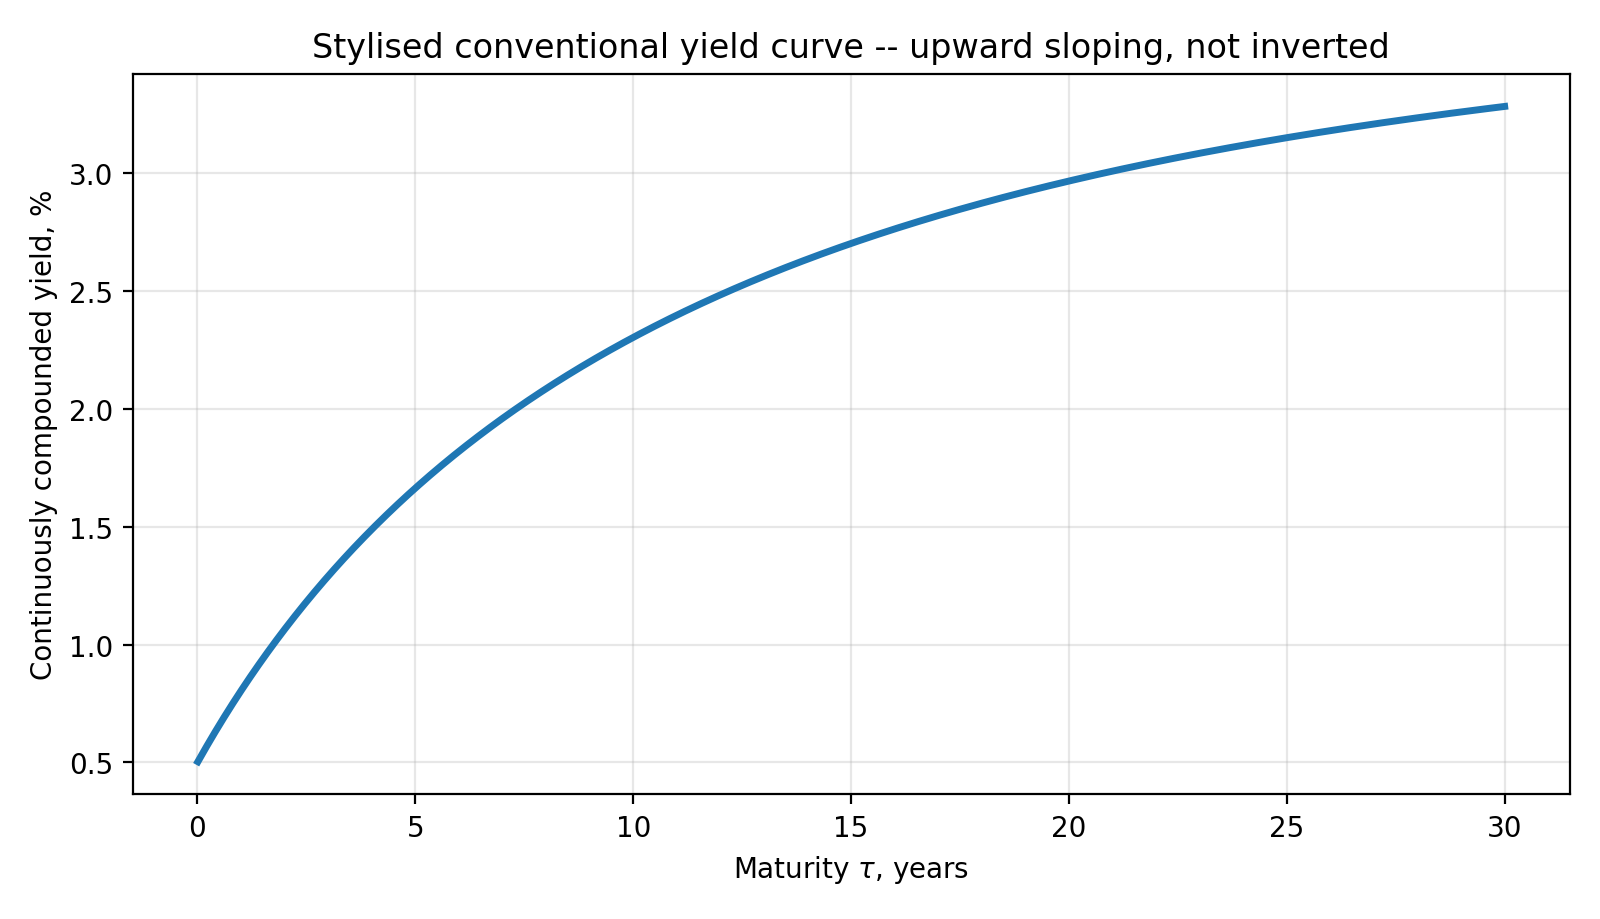
\includegraphics[width=0.95\textwidth]{fig_conventional_yield_curve_first_example.png}
    \caption{Stylised upward-sloping conventional yield curve under the general
    \(r\)-branch.  The parameter set is \(x_{\infty}=4.00\%\),
    \(x_{t_{0},t_{0}}=0.50\%\), \(a=0.70\), and \(r=0.30\), with
    \(t=t_{0}\).  The curve is upward sloping and non-inverted.}
    \label{fig:conventional-yield-upward-example}
\end{figure}

\begin{figure}[p]
    \centering
    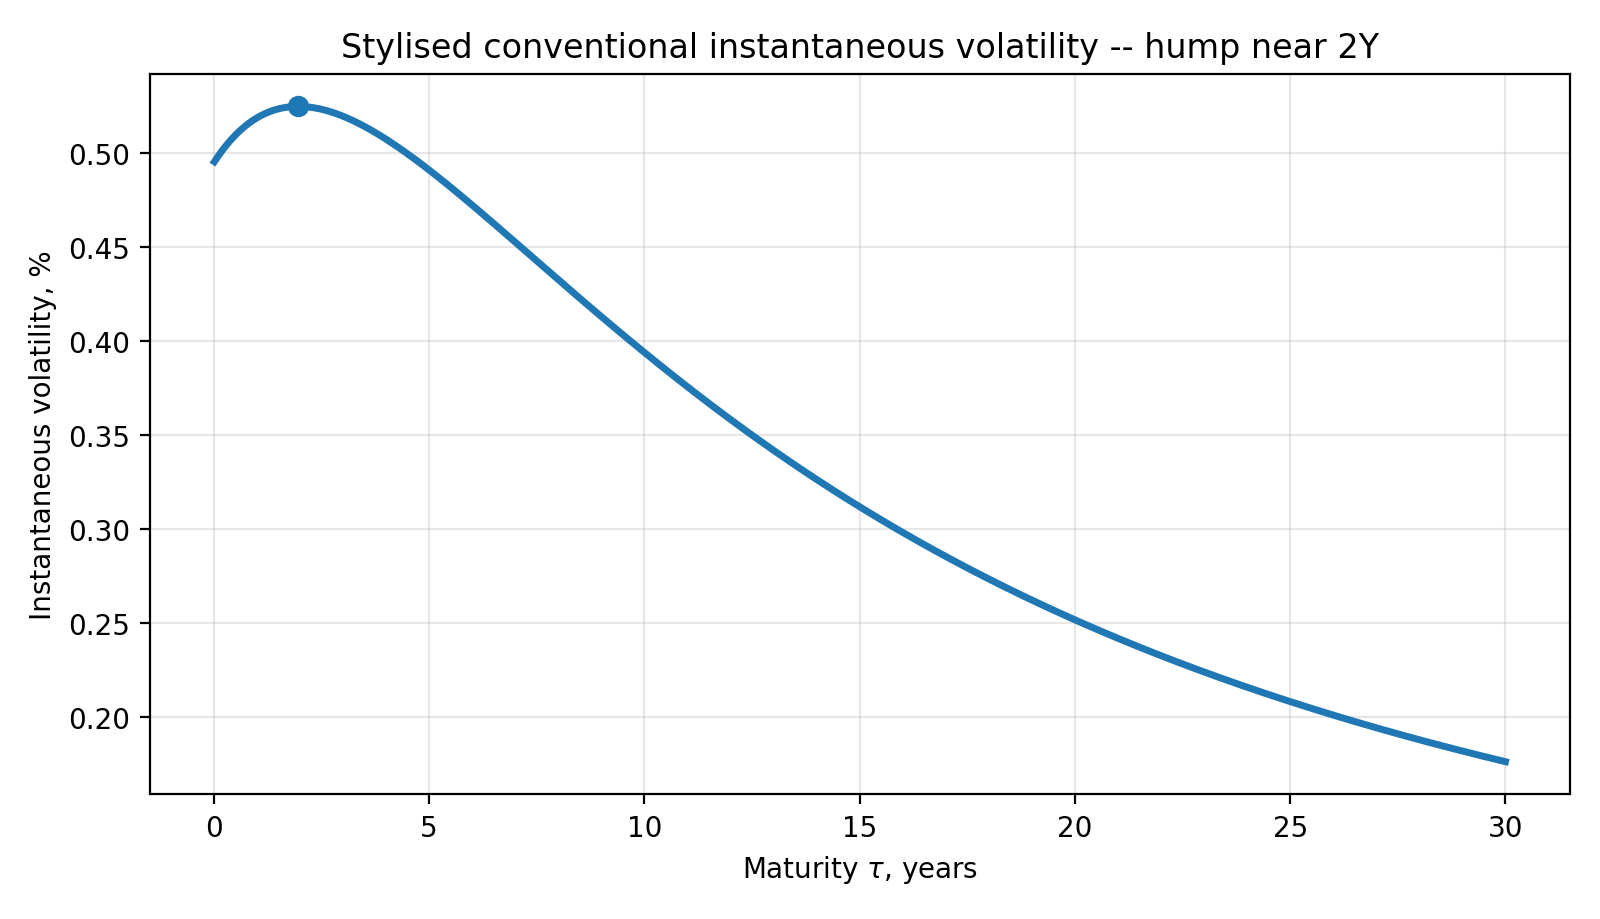
\includegraphics[width=0.95\textwidth]{fig_conventional_vol_hump_first_example.png}
    \caption{Stylised conventional-rate instantaneous volatility under the same
    parameter set as Figure~\ref{fig:conventional-yield-upward-example}.  The
    volatility is non-zero for finite maturity and has an interior hump close
    to the two-year maturity, despite the underlying conventional yield curve
    being upward sloping rather than inverted.}
    \label{fig:conventional-volatility-hump-example}
\end{figure}
\clearpage

% ------------------------------------------------------------
\subsection{Risk Management and Stress Testing}
\label{subsec:risk}

Because the maturity-indexed equilibrium density is heavy-tailed and
strictly positive on its shifted support, stress scenarios may
incorporate large rate moves drawn from the generalized shifted
inverse-gamma law. Perturbations in \((a,r,x_{\infty})\) provide a
coherent way to stress-test mean reversion, maturity decay, equilibrium
regime assumptions, and hump risk. The variance-rate formula
\eqref{eq:var-final} also identifies maturities at which local
uncertainty is amplified by the interaction of the two exponential
loadings.

% ------------------------------------------------------------
\subsection{Pricing Interest-Rate--Dependent Claims}
\label{subsec:pricing}

Under a risk-neutral measure, the drift adjusts to incorporate market
prices of risk, while the diffusion remains affine in the shifted state.
The shifted positivity structure makes the model suitable for pricing
caps, floors, swaptions, and other interest-rate--dependent claims. The
two-exponential forward-curve representation gives a tractable basis for
semi-closed-form pricing and calibration while preserving one-factor
stochastic dynamics.
% ------------------------------------------------------------
% Appendices
% ------------------------------------------------------------
\begin{appendices}
\section{Technical Derivations for Section 3}
\label{appendix:A}

This appendix provides full derivations of the structural results in
Section~\ref{sec:framework}. All proofs follow a clear step-by-step
format.

% ============================================================
\subsection{Proof of Statement~\ref{stmt:affineforms}}
\label{appendix:A1}
\medskip
\noindent\textbf{Step 1: Expand the KFE.}  
From \eqref{eq:kfe-f-g},
\begin{equation}
\frac{\partial\varphi}{\partial t}
=
g^{2}\varphi_{xx}
+
\bigl(2(g^{2})_{x}+f\bigr)\varphi_{x}
+
\bigl((g^{2})_{xx}+f_{x}\bigr)\varphi.
\tag{A.1.1}
\end{equation}
Equivalently, since \((g^{2})_{x}=2g g_{x}\),
\[
\frac{\partial\varphi}{\partial t}
=
g^{2}\varphi_{xx}
+
(4g g_{x}+f)\varphi_{x}
+
\bigl((g^{2})_{xx}+f_{x}\bigr)\varphi.
\]

\medskip
\noindent\textbf{Step 2: Apply rolling--maturity invariance (Axiom 2).}  
Axiom~2 implies that the coefficients depend on calendar time only through
remaining maturity \(\tau=T-t\). Hence there exist functions \(F\) and
\(G\) such that
\begin{equation}
f(x,t,T)=F(x,\tau),
\qquad
g(x,t,T)=G(x,\tau),
\qquad \tau=T-t.
\tag{A.1.2}
\end{equation}

\medskip
\noindent\textbf{Step 3: Impose the affine-closure hypothesis.}  
Assume that for each fixed \(\tau\),
\begin{equation}
\partial_{xx}G(x,\tau)=0,
\tag{A.1.3}\label{eq:A13}
\end{equation}
and that the net probability flux is affine in \(x\):
\begin{equation}
\partial_x\!\bigl(G(x,\tau)^2\bigr)+F(x,\tau)=A(\tau)x+B(\tau)
\tag{A.1.4}\label{eq:A14}
\end{equation}
for some functions \(A(\tau)\) and \(B(\tau)\).

\medskip
\noindent\textbf{Step 4: Solve for the diffusion.}  
Equation \eqref{eq:A13} implies that \(G\) is affine in \(x\). Therefore
there exist functions \(a(\tau)\) and \(b(\tau)\) such that
\begin{equation}
G(x,\tau)=a(\tau)x+b(\tau).
\tag{A.1.5}\label{eq:A15}
\end{equation}

\medskip
\noindent\textbf{Step 5: Solve for the drift.}  
Substituting \eqref{eq:A15} into \eqref{eq:A14} gives
\[
F(x,\tau)
=
A(\tau)x+B(\tau)-\partial_x\!\bigl(G(x,\tau)^2\bigr).
\]
But
\[
\partial_x\!\bigl(G(x,\tau)^2\bigr)
=
2a(\tau)\bigl(a(\tau)x+b(\tau)\bigr),
\]
which is affine in \(x\). Hence \(F\) is affine in \(x\) as well, so there
exist functions \(a_1(\tau)\) and \(b_1(\tau)\) such that
\begin{equation}
F(x,\tau)=a_1(\tau)x+b_1(\tau).
\tag{A.1.6}\label{eq:A16}
\end{equation}

\medskip
\noindent\textbf{Step 6: Return to the original notation.}  
Using \(\tau=T-t\), equations \eqref{eq:A15} and \eqref{eq:A16} become
\[
g(x,t,T)=a(T-t)x+b(T-t),
\qquad
f(x,t,T)=a_1(T-t)x+b_1(T-t).
\]
Thus both diffusion and drift are affine in the IRFR state \(x\), which
establishes Statement~\ref{stmt:affineforms}.
% ============================================================
% ============================================================
\subsection{Proof of Statement \ref{stmt:eqrelation}}
\label{appendix:A2}

\textbf{Goal.}  
Derive the equilibrium drift--diffusion relations
\eqref{eq:eqdrift}--\eqref{eq:eqdiffusion}.

\medskip
\noindent\textbf{Step 1: Equilibrium identity.}  
Under Axiom 3, the equilibrium IRFR depends only on time-to-maturity, so that
\[
x_{e,T-t}=x_{e,\tau}, \qquad \tau:=T-t.
\]
Hence
\[
\frac{\partial x_{e,T-t}}{\partial t}
=
-\,x'_{e,\tau}.
\tag{A.2.12}
\]

\medskip
\noindent\textbf{Step 2: First-moment evolution.}  
From the Fokker--Planck equation, multiplying by \(x\), integrating over
\(x\in[x_{\min},\infty)\), and assuming the boundary terms vanish, gives
\[
\frac{\partial}{\partial t}\mathbb{E}[x_{t,T}]
=
-\mathbb{E}[f(x,t,T)].
\tag{A.2.13}
\]
Using the affine drift form from Statement~\ref{stmt:affineforms},
\[
f(x,t,T)=a_1(\tau)x+b_1(\tau),
\tag{A.2.14}\label{eq:A214}
\]
it follows that
\[
\frac{\partial}{\partial t}\mathbb{E}[x_{t,T}]
=
-\,a_1(\tau)\mathbb{E}[x_{t,T}] - b_1(\tau).
\tag{A.2.15}\label{eq:A215}
\]

\medskip
\noindent\textbf{Step 3: Impose equilibrium.}  
At equilibrium,
\[
\mathbb{E}[x_{t,T}]=x_{e,\tau},
\]
so \eqref{eq:A215} becomes
\[
\frac{\partial x_{e,\tau}}{\partial t}
=
-\,a_1(\tau)x_{e,\tau}-b_1(\tau).
\tag{A.2.16}
\]
Using \(\partial_t x_{e,\tau}=-x'_{e,\tau}\), we obtain
\[
-\,x'_{e,\tau}
=
-\,a_1(\tau)x_{e,\tau}-b_1(\tau),
\]
hence
\[
b_1(\tau)
=
-\,a_1(\tau)x_{e,\tau}+x'_{e,\tau}.
\tag{A.2.17}\label{eq:A217}
\]

\medskip
\noindent\textbf{Step 4: Drift relation.}  
Substituting \eqref{eq:A217} into \eqref{eq:A214} yields
\[
f(x,t,T)
=
a_1(\tau)x-a_1(\tau)x_{e,\tau}+x'_{e,\tau},
\]
that is,
\[
f(x,t,T)
=
a_1(\tau)\bigl(x-x_{e,\tau}\bigr)+x'_{e,\tau}.
\tag{A.2.18}
\]
Identifying \(x\) with the state variable \(x_{t,T}\) gives
\eqref{eq:eqdrift}.

\medskip
\noindent\textbf{Step 5: Diffusion relation.}  
Using the affine diffusion form from Statement~\ref{stmt:affineforms},
\[
g(x,t,T)=a(\tau)x+b(\tau),
\tag{A.2.19}
\]
together with the proportionality hypothesis
\[
b(\tau)=\frac{a(\tau)}{a_1(\tau)}\,b_1(\tau),
\tag{A.2.20}
\]
and substituting \eqref{eq:A217}, one finds
\[
b(\tau)
=
\frac{a(\tau)}{a_1(\tau)}
\Bigl(-\,a_1(\tau)x_{e,\tau}+x'_{e,\tau}\Bigr)
=
-\,a(\tau)x_{e,\tau}+\frac{a(\tau)}{a_1(\tau)}x'_{e,\tau}.
\tag{A.2.21}
\]
Therefore
\[
g(x,t,T)
=
a(\tau)x-a(\tau)x_{e,\tau}+\frac{a(\tau)}{a_1(\tau)}x'_{e,\tau},
\]
i.e.
\[
g(x,t,T)
=
a(\tau)\bigl(x-x_{e,\tau}\bigr)
+
\frac{a(\tau)}{a_1(\tau)}x'_{e,\tau}.
\tag{A.2.22}
\]
Identifying \(x\) with the state variable \(x_{t,T}\) gives
\eqref{eq:eqdiffusion}.

\medskip
This proves Statement~\ref{stmt:eqrelation}.
% ============================================================
\subsection{Proof of Statement \ref{stmt:expectation}}
\label{appendix:A3}

\textbf{Goal.}
Show that, for fixed maturity \(T\),
\[
\mathbb{E}[x_{t,T}]
=
x_{e,T-t}
+
\left(x_{t_0,T}-x_{e,T-t_0}\right)e^{-a_1(t-t_0)}.
\]

\medskip
\noindent\textbf{Step 1: Start from the expectation dynamics.}
By Statement \ref{stmt:expectation}, the expected forward rate satisfies
\[
\frac{\partial \mathbb{E}[x_{t,T}]}{\partial t}
=
-a_1\bigl(\mathbb{E}[x_{t,T}] - x_{e,T-t}\bigr)
+
\frac{\partial x_{e,T-t}}{\partial t},
\]
where \(a_1>0\) is constant.

\medskip
\noindent\textbf{Step 2: Define the deviation from equilibrium.}
Let
\[
z(t):=\mathbb{E}[x_{t,T}] - x_{e,T-t}.
\]
Then
\[
\frac{dz(t)}{dt}
=
\frac{\partial \mathbb{E}[x_{t,T}]}{\partial t}
-
\frac{\partial x_{e,T-t}}{\partial t}.
\]
Substituting the expectation dynamics gives
\[
\frac{dz(t)}{dt}
=
-a_1\bigl(\mathbb{E}[x_{t,T}] - x_{e,T-t}\bigr)
=
-a_1 z(t).
\]

\medskip
\noindent\textbf{Step 3: Solve the differential equation.}
The solution is
\[
z(t)=z(t_0)e^{-a_1(t-t_0)}.
\]
Hence
\[
\mathbb{E}[x_{t,T}] - x_{e,T-t}
=
\left(\mathbb{E}[x_{t_0,T}] - x_{e,T-t_0}\right)e^{-a_1(t-t_0)}.
\]

\medskip
\noindent\textbf{Step 4: Apply the initial condition.}
At time \(t_0\), the forward rate is known, so
\[
\mathbb{E}[x_{t_0,T}] = x_{t_0,T}.
\]
Therefore
\[
\mathbb{E}[x_{t,T}] - x_{e,T-t}
=
\left(x_{t_0,T} - x_{e,T-t_0}\right)e^{-a_1(t-t_0)}.
\]
Rearranging yields
\begin{equation}
\mathbb{E}[x_{t,T}]
=
x_{e,T-t}
+
\left(x_{t_0,T}-x_{e,T-t_0}\right)e^{-a_1(t-t_0)}.
\tag{A.3.1}\label{eq:A31}
\end{equation}

This proves Statement \ref{stmt:expectation}.
% ============================================================
% ============================================================
\subsection{Derivation of the Baseline Drift--Diffusion Identification}
\label{appendix:A4}

\textbf{Goal.}
Derive the variance equation that motivates the baseline identification
\[
a_1=a^2.
\]
The calculation below shows exactly where an independent drift scale would enter
the second-moment dynamics.

\medskip
\noindent\textbf{Step 1: Start from the variance dynamics.}
Let
\[
V(t,T):=\operatorname{Var}(x_{t,T}).
\]
From the affine diffusion specification, the forward rate satisfies
\[
dx_{t,T}
=
\bigl(-a_1x_{t,T}+a_1x_{e,T-t}+\partial_t x_{e,T-t}\bigr)\,dt
+
\bigl(a x_{t,T}+b(T-t)\bigr)\,dW_t,
\]
where, by Statement~\ref{stmt:eqrelation},
\[
b(T-t)=-a\,x_{e,T-t}+\frac{1}{a}x'_{e,T-t}.
\]

\medskip
\noindent\textbf{Step 2: Derive the second-moment equation.}
Applying It\^o's formula to \(x_{t,T}^2\) and taking expectations gives
\begin{align}
\frac{\partial}{\partial t}\mathbb{E}[x_{t,T}^2]
&=
2\,\mathbb{E}\!\left[x_{t,T}
\bigl(-a_1x_{t,T}+a_1x_{e,T-t}+\partial_t x_{e,T-t}\bigr)\right]
+
\mathbb{E}\!\left[\bigl(a x_{t,T}+b(T-t)\bigr)^2\right]
\nonumber\\
&=
(-2a_1+a^2)\mathbb{E}[x_{t,T}^2]
+
\bigl(2a_1x_{e,T-t}+2\partial_t x_{e,T-t}+2ab(T-t)\bigr)\mathbb{E}[x_{t,T}]
+
b(T-t)^2.
\tag{A.4.1}\label{eq:A41}
\end{align}

\medskip
\noindent\textbf{Step 3: Pass from the second moment to the variance.}
Since
\[
V(t,T)=\mathbb{E}[x_{t,T}^2]-\mathbb{E}[x_{t,T}]^2,
\]
differentiate with respect to \(t\):
\[
\frac{\partial V}{\partial t}
=
\frac{\partial}{\partial t}\mathbb{E}[x_{t,T}^2]
-
2\,\mathbb{E}[x_{t,T}]
\frac{\partial}{\partial t}\mathbb{E}[x_{t,T}].
\]
Using Statement~\ref{stmt:expectation},
\[
\frac{\partial}{\partial t}\mathbb{E}[x_{t,T}]
=
-a_1\bigl(\mathbb{E}[x_{t,T}]-x_{e,T-t}\bigr)
+
\partial_t x_{e,T-t},
\tag{A.4.2}\label{eq:A42}
\]
and substituting \eqref{eq:A41} and \eqref{eq:A42}, the mixed terms cancel. This yields
\[
\frac{\partial V}{\partial t}
=
2(a^2-a_1)V
+
\bigl(a\,x_{e,T-t}+b(T-t)\bigr)^2.
\tag{A.4.3}\label{eq:A43}
\]

\medskip
\noindent\textbf{Step 4: Use the equilibrium diffusion relation.}
From Statement~\ref{stmt:eqrelation},
\[
b(T-t)=-a\,x_{e,T-t}+\frac{1}{a}x'_{e,T-t}.
\]
Hence
\[
a\,x_{e,T-t}+b(T-t)=\frac{1}{a}x'_{e,T-t},
\]
so \eqref{eq:A43} becomes
\[
\frac{\partial V}{\partial t}
=
2(a^2-a_1)V
+
\frac{1}{a^2}\bigl(x'_{e,T-t}\bigr)^2.
\tag{A.4.4}\label{eq:A44}
\]

\medskip
\noindent\textbf{Step 5: Identify the baseline one-scale case.}
Under equilibrium transport, admissible term-structure objects depend on calendar
time and maturity through
\[
\tau:=T-t.
\]
If the variance is written as \(V(t,T)=\widetilde V(\tau)\), then
\[
\frac{\partial V}{\partial t}=-\widetilde V'(\tau),
\]
and \eqref{eq:A44} becomes
\[
-\widetilde V'(\tau)
=
2(a^2-a_1)\widetilde V(\tau)
+
\frac{1}{a^2}\bigl(x_e'(\tau)\bigr)^2.
\tag{A.4.5}\label{eq:A45}
\]
Equation \eqref{eq:A45} displays the structural choice clearly. If
\(a_1\neq a^2\), the variance equation carries an additional homogeneous
component proportional to \(\widetilde V(\tau)\), introducing a second decay scale
beyond the diffusion scale \(a\). The baseline model rules out this additional
independent variance scale by imposing the one-scale identification
\[
a_1=a^2.
\tag{A.4.6}\label{eq:A46}
\]
Under this baseline identification, \eqref{eq:A44} reduces to
\[
\frac{\partial V}{\partial t}
=
\frac{1}{a^2}\bigl(x'_{e,T-t}\bigr)^2,
\]
so the variance production is governed by the same structural scale used in the
drift--diffusion specification.

This establishes the baseline identification used in Statement~\ref{stmt:a1eqasq}.

% ============================================================
\subsection{Proof of Statement~\ref{stmt:interim}}
\label{appendix:A5}

\textbf{Goal.}
Show that once the baseline exponential equilibrium specification is
imposed, consistency of the equilibrium relations determines the interim
forms \eqref{eq:interim-f}--\eqref{eq:interim-g}.

\medskip
\noindent\textbf{Step 1: Start from the equilibrium drift and diffusion relations.}

From Appendix~\ref{appendix:A2}, the equilibrium relations are
\begin{align}
f(x,t,T)
&=
a_1 x_{t,T}
-
a_1 x_{e,T-t}
-
\frac{\partial x_{e,T-t}}{\partial t},
\tag{A.5.1a}\label{eq:A5eqdrift}
\\[0.4em]
g(x,t,T)
&=
a x_{t,T}
-
a x_{e,T-t}
-
\frac{a}{a_1}\frac{\partial x_{e,T-t}}{\partial t}.
\tag{A.5.1b}\label{eq:A5eqdiff}
\end{align}
Since \(\tau=T-t\), we have
\[
-\frac{\partial x_{e,T-t}}{\partial t}
=
\frac{\partial x_{e,T-t}}{\partial T}.
\]
Using the baseline identification \(a_1=a^2\), this becomes
\begin{align}
f(x,t,T)
&=
a^{2}x_{t,T}
-
a^{2}x_{e,T-t}
+
\frac{\partial x_{e,T-t}}{\partial T},
\tag{A.5.2a}\label{eq:A5fpre}
\\[0.4em]
g(x,t,T)
&=
a x_{t,T}
-
a x_{e,T-t}
+
\frac{1}{a}\frac{\partial x_{e,T-t}}{\partial T}.
\tag{A.5.2b}\label{eq:A5gpre}
\end{align}

\medskip
\noindent\textbf{Step 2: Impose the baseline exponential equilibrium specification.}

At this stage, no unique functional form for \(x_{e,T-t}\) has been
derived. We now impose the baseline exponential equilibrium specification
used in the main text:
\begin{equation}
x_{e,T-t}
=
x_{\infty}+A e^{-\lambda^{2}(T-t)}.
\tag{A.5.3}\label{eq:A5xeTT}
\end{equation}
Equivalently, in the maturity variable \(\tau=T-t\),
\begin{equation}
x_{e,\tau}=x_{\infty}+A e^{-\lambda^{2}\tau}.
\tag{A.5.4}\label{eq:A5xe}
\end{equation}
Differentiating \eqref{eq:A5xeTT} with respect to \(T\) yields
\begin{equation}
\frac{\partial x_{e,T-t}}{\partial T}
=
-\lambda^{2}A e^{-\lambda^{2}(T-t)}.
\tag{A.5.5}\label{eq:A5xediff}
\end{equation}

\medskip
\noindent\textbf{Step 3: Substitute into the equilibrium relations.}

Substituting \eqref{eq:A5xeTT} and \eqref{eq:A5xediff} into
\eqref{eq:A5fpre} gives
\begin{align}
f(x,t,T)
&=
a^{2}x_{t,T}
-
a^{2}\!\left(x_{\infty}+A e^{-\lambda^{2}(T-t)}\right)
-
\lambda^{2}A e^{-\lambda^{2}(T-t)}
\nonumber\\
&=
a^{2}x_{t,T}
-
a^{2}x_{\infty}
-
(\lambda^{2}+a^{2})A e^{-\lambda^{2}(T-t)}.
\tag{A.5.6}\label{eq:A51}
\end{align}
Likewise, substituting \eqref{eq:A5xeTT} and \eqref{eq:A5xediff} into
\eqref{eq:A5gpre} gives
\begin{align}
g(x,t,T)
&=
a x_{t,T}
-
a\!\left(x_{\infty}+A e^{-\lambda^{2}(T-t)}\right)
-
\frac{\lambda^{2}}{a}A e^{-\lambda^{2}(T-t)}
\nonumber\\
&=
a x_{t,T}
-
a x_{\infty}
-
\left(a+\frac{\lambda^{2}}{a}\right)
A e^{-\lambda^{2}(T-t)}.
\tag{A.5.7}\label{eq:A52}
\end{align}

\medskip
\noindent\textbf{Conclusion.}

Thus, once the baseline exponential equilibrium curve is imposed,
consistency of the equilibrium drift and diffusion relations yields the
interim forms \eqref{eq:interim-f}--\eqref{eq:interim-g}. This is a
conditional identification result, not a uniqueness statement about all
admissible equilibrium curves.

% ============================================================
\subsection{Proof of Statement~\ref{stmt:interim_inst_variance}}
\label{appendix:A6}

Goal. Derive the instantaneous variance-rate implied by the interim drift and diffusion
forms obtained under the baseline exponential equilibrium specification.

Step 1: Moment identities from the KFE.

The Kolmogorov Forward Equation is
\[
\frac{\partial \varphi}{\partial t}
=
\frac{\partial^2}{\partial x^2}\left(g^2(x,t,T)\varphi\right)
+
\frac{\partial}{\partial x}\left(f(x,t,T)\varphi\right).
\]
Assuming the boundary terms vanish, multiplication by \(x\) and integration over the
state space gives
\[
\frac{\partial}{\partial t}\mathbb E[x_{t,T}]
=
-\mathbb E[f(x_{t,T},t,T)].
\]
Likewise, multiplication by \(x^2\) and integration by parts gives
\[
\frac{\partial}{\partial t}\mathbb E[x_{t,T}^2]
=
-2\mathbb E[x_{t,T}f(x_{t,T},t,T)]
+
2\mathbb E[g^2(x_{t,T},t,T)].
\]

Step 2: Pass from second moments to variance.

Let
\[
m(t,T):=\mathbb E[x_{t,T}],
\qquad
V(t,T):=\operatorname{Var}(x_{t,T}).
\]
Since
\[
V(t,T)=\mathbb E[x_{t,T}^2]-m(t,T)^2,
\]
we obtain
\[
\frac{\partial V}{\partial t}
=
-2\mathbb E[x_{t,T}f(x_{t,T},t,T)]
+
2\mathbb E[g^2(x_{t,T},t,T)]
+
2m(t,T)\mathbb E[f(x_{t,T},t,T)].
\]

Step 3: Use the affine forms of \(f\) and \(g\).

Under the interim baseline specification,
\[
f(x,t,T)
=
a^2x
-
a^2x_\infty
-
(\lambda^2+a^2)Ae^{-\lambda^2(T-t)},
\]
and
\[
g(x,t,T)
=
ax
-
ax_\infty
-
\left(a+\frac{\lambda^2}{a}\right)Ae^{-\lambda^2(T-t)}.
\]
Write these as
\[
f(x,t,T)=a^2x+\beta(t,T),
\qquad
g(x,t,T)=ax+\gamma(t,T),
\]
where
\[
\beta(t,T)
=
-a^2x_\infty
-
(\lambda^2+a^2)Ae^{-\lambda^2(T-t)},
\]
and
\[
\gamma(t,T)
=
-ax_\infty
-
\left(a+\frac{\lambda^2}{a}\right)Ae^{-\lambda^2(T-t)}.
\]

Since \(f\) is affine,
\[
\mathbb E[f(x_{t,T},t,T)]
=
a^2m(t,T)+\beta(t,T),
\]
and
\[
\mathbb E[x_{t,T}f(x_{t,T},t,T)]
=
a^2\mathbb E[x_{t,T}^2]+\beta(t,T)m(t,T).
\]
Therefore,
\[
-2\mathbb E[x_{t,T}f(x_{t,T},t,T)]
+
2m(t,T)\mathbb E[f(x_{t,T},t,T)]
=
-2a^2V(t,T).
\]

For the diffusion term,
\[
\mathbb E[g^2(x_{t,T},t,T)]
=
\mathbb E[(ax_{t,T}+\gamma(t,T))^2].
\]
Hence
\[
\mathbb E[g^2(x_{t,T},t,T)]
=
a^2V(t,T)
+
\left(am(t,T)+\gamma(t,T)\right)^2.
\]
Substituting into the variance equation gives
\[
\frac{\partial V}{\partial t}
=
-2a^2V(t,T)
+
2a^2V(t,T)
+
2\left(am(t,T)+\gamma(t,T)\right)^2.
\]
The variance terms cancel, so
\[
\frac{\partial}{\partial t}\operatorname{Var}(x_{t,T})
=
2\left(am(t,T)+\gamma(t,T)\right)^2.
\]

Step 4: Substitute the mean branch.

From Statement 3.3, under the baseline exponential equilibrium curve,
\[
m(t,T)
=
x_\infty
+
Ae^{-\lambda^2(T-t)}
+
D(t,T),
\]
where
\[
D(t,T)
:=
\left(
x_{t_0,T}
-
x_\infty
-
Ae^{-\lambda^2(T-t_0)}
\right)
e^{-a^2(t-t_0)}.
\]
Therefore
\[
am(t,T)+\gamma(t,T)
=
a\left(x_\infty+Ae^{-\lambda^2(T-t)}+D(t,T)\right)
-
ax_\infty
-
\left(a+\frac{\lambda^2}{a}\right)Ae^{-\lambda^2(T-t)}.
\]
After cancellation,
\[
am(t,T)+\gamma(t,T)
=
aD(t,T)
-
\frac{\lambda^2}{a}Ae^{-\lambda^2(T-t)}.
\]
Thus,
\[
\frac{\partial}{\partial t}\operatorname{Var}(x_{t,T})
=
2\left(
aD(t,T)
-
\frac{\lambda^2}{a}Ae^{-\lambda^2(T-t)}
\right)^2.
\]

Step 5: Expanded final form.

Substituting the definition of \(D(t,T)\), the variance-rate formula is
\[
\boxed{
\frac{\partial}{\partial t}\operatorname{Var}(x_{t,T})
=
2\left[
a\left(
x_{t_0,T}
-
x_\infty
-
Ae^{-\lambda^2(T-t_0)}
\right)
e^{-a^2(t-t_0)}
-
\frac{\lambda^2}{a}Ae^{-\lambda^2(T-t)}
\right]^2.
}
\label{eq:interim_inst_variance}\tag{A.6.1}
\]


This proves Statement 3.6.
% ============================================================
\subsection{Proof of Statement~\ref{stmt:msnr}}
\label{appendix:A7}

Goal. Derive the market signal-to-noise ratio.

Step 1: Start from the variance rate.

From Appendix A.6, the instantaneous variance-rate is
\[
\frac{\partial}{\partial t}\operatorname{Var}(x_{t,T})
=
2\left(
aD(t,T)
-
\frac{\lambda^2}{a}Ae^{-\lambda^2(T-t)}
\right)^2,
\]
where
\[
D(t,T)
:=
\left(
x_{t_0,T}
-
x_\infty
-
Ae^{-\lambda^2(T-t_0)}
\right)
e^{-a^2(t-t_0)}.
\]
Hence the instantaneous noise scale is
\[
\sqrt{
\frac{\partial}{\partial t}\operatorname{Var}(x_{t,T})
}
=
\sqrt{2}
\left|
aD(t,T)
-
\frac{\lambda^2}{a}Ae^{-\lambda^2(T-t)}
\right|.
\]

Step 2: Evaluate the drift on the mean branch.

From Appendix A.5, the interim drift is
\[
f(x,t,T)
=
a^2x
-
a^2x_\infty
-
(\lambda^2+a^2)Ae^{-\lambda^2(T-t)}.
\]
The mean branch is
\[
m(t,T)
=
x_\infty
+
Ae^{-\lambda^2(T-t)}
+
D(t,T).
\]
Evaluating the drift along this mean branch gives
\[
f(m(t,T),t,T)
=
a^2\left(
x_\infty
+
Ae^{-\lambda^2(T-t)}
+
D(t,T)
\right)
-
a^2x_\infty
-
(\lambda^2+a^2)Ae^{-\lambda^2(T-t)}.
\]
After cancellation,
\[
f(m(t,T),t,T)
=
a^2D(t,T)
-
\lambda^2Ae^{-\lambda^2(T-t)}.
\]
Equivalently,
\[
f(m(t,T),t,T)
=
a\left(
aD(t,T)
-
\frac{\lambda^2}{a}Ae^{-\lambda^2(T-t)}
\right).
\]
Therefore the instantaneous signal scale, defined as the magnitude of the drift along the
mean branch, is
\[
|f(m(t,T),t,T)|
=
a
\left|
aD(t,T)
-
\frac{\lambda^2}{a}Ae^{-\lambda^2(T-t)}
\right|.
\]

Step 3: Form the ratio.

The Market Signal-to-Noise Ratio is therefore
\[
\mathrm{MSNR}
=
\frac{|f(m(t,T),t,T)|}
{\sqrt{\frac{\partial}{\partial t}\operatorname{Var}(x_{t,T})}}
=
\frac{
a
\left|
aD(t,T)
-
\frac{\lambda^2}{a}Ae^{-\lambda^2(T-t)}
\right|
}{
\sqrt{2}
\left|
aD(t,T)
-
\frac{\lambda^2}{a}Ae^{-\lambda^2(T-t)}
\right|
}.
\]
Thus,
\[
\boxed{
\mathrm{MSNR}
=
\frac{a}{\sqrt{2}}.
}
\]

Step 4: Expanded form.

Equivalently, substituting the definition of \(D(t,T)\), the instantaneous signal scale is
\[
|f(m(t,T),t,T)|
=
a\left|
a\left(
x_{t_0,T}
-
x_\infty
-
Ae^{-\lambda^2(T-t_0)}
\right)
e^{-a^2(t-t_0)}
-
\frac{\lambda^2}{a}Ae^{-\lambda^2(T-t)}
\right|,
\]
and the instantaneous noise scale is
\[
\sqrt{
\frac{\partial}{\partial t}\operatorname{Var}(x_{t,T})
}
=
\sqrt{2}
\left|
a\left(
x_{t_0,T}
-
x_\infty
-
Ae^{-\lambda^2(T-t_0)}
\right)
e^{-a^2(t-t_0)}
-
\frac{\lambda^2}{a}Ae^{-\lambda^2(T-t)}
\right|.
\]
Their ratio is therefore again
\[
\boxed{
\mathrm{MSNR}=\frac{a}{\sqrt{2}}.
}
\]
This proves Statement 3.7.
% ============================================================



% ============================================================
% Appendix B
%==============================================================

\section{KFE Solution in the Equilibrium Regime}
\label{appendix:B}

% ------------------------------------------------------------
\subsection{Full Frobenius Proof of the equilibrium regime PDF}
\label{appendix:B1}

We begin from the transformed KFE in the shifted variable
\[
\widetilde{x}_{t,T}
=
x_{t,T}
-
x_{\infty}\!\left(1-e^{-\lambda^{2}(T-t)}\right),
\]
so that the equilibrium mean has been removed, but without yet imposing any
relation between \(\lambda\) and \(a\). In these coordinates the KFE takes the form
\begin{equation}
\frac{\partial \varphi}{\partial t}
=
a^{2}\widetilde{x}_{t,T}^{2}\varphi_{\widetilde{x}_{t,T}\widetilde{x}_{t,T}}
+
5a^{2}\widetilde{x}_{t,T}\,\varphi_{\widetilde{x}_{t,T}}
+
3a^{2}\varphi
-
\lambda^{2}x_{\infty}e^{-\lambda^{2}(T-t)}\varphi_{\widetilde{x}_{t,T}}.
\tag{B.1.1}\label{eq:B11}
\end{equation}

To analyse the singular structure at \(\widetilde{x}_{t,T}=0\), introduce the reciprocal
variable
\[
z=\frac{1}{\widetilde{x}_{t,T}},
\qquad
z_{\widetilde{x}_{t,T}}=-z^{2},
\qquad
z_{\widetilde{x}_{t,T}\widetilde{x}_{t,T}}=2z^{3}.
\]
Using
\[
\varphi_{\widetilde{x}_{t,T}}=-z^{2}\varphi_{z},
\qquad
\varphi_{\widetilde{x}_{t,T}\widetilde{x}_{t,T}}
=
z^{4}\varphi_{zz}+2z^{3}\varphi_{z},
\]
equation \eqref{eq:B11} becomes
\begin{equation}
\frac{\partial \varphi}{\partial t}
=
a^{2}z^{2}\varphi_{zz}
-
3a^{2}z\varphi_{z}
+
3a^{2}\varphi
+
\lambda^{2}x_{\infty}e^{-\lambda^{2}(T-t)}z^{2}\varphi_{z}.
\tag{B.1.2}\label{eq:B12}
\end{equation}

\medskip
\noindent\textbf{Step 1: Frobenius expansion.}

Seek a Frobenius series of the form
\[
\varphi(z,t,T)=\sum_{i=0}^{\infty} c_i(t)\,z^{i+m}.
\]
Then
\[
\varphi_z
=
\sum_{i=0}^{\infty}(i+m)c_i(t)\,z^{i+m-1},
\qquad
\varphi_{zz}
=
\sum_{i=0}^{\infty}(i+m)(i+m-1)c_i(t)\,z^{i+m-2}.
\]
Substituting into \eqref{eq:B12} and matching coefficients of \(z^{i+m}\) yields
\begin{equation}
\frac{\partial c_i}{\partial t}
=
a^{2}(i+m-1)(i+m-3)c_i
+
\lambda^{2}x_{\infty}e^{-\lambda^{2}(T-t)}(i+m-1)c_{i-1},
\tag{B.1.3}\label{eq:B13}
\end{equation}
with \(c_{-1}\equiv 0\).

\medskip
\noindent\textbf{Step 2: Separate the time dependence.}

Write
\[
c_i(t)=c_i^{*}\,x_{\infty}^{\,i+n}e^{-(i+n)\lambda^{2}(T-t)}.
\]
Then
\[
\frac{\partial c_i}{\partial t}=(i+n)\lambda^{2}c_i(t).
\]
Substituting into \eqref{eq:B13} and cancelling the common factor
\(x_{\infty}^{\,i+n}e^{-(i+n)\lambda^{2}(T-t)}\) gives
\[
(i+n)\lambda^{2}c_i^{*}
=
a^{2}(i+m-1)(i+m-3)c_i^{*}
+
\lambda^{2}(i+m-1)c_{i-1}^{*}.
\]
At \(i=0\), since \(c_{-1}^{*}=0\), this reduces to the indicial relation
\begin{equation}
n\,\frac{\lambda^{2}}{a^{2}}=(m-1)(m-3).
\tag{B.1.4}\label{eq:B14}
\end{equation}
For \(i\ge 1\), subtracting \eqref{eq:B14} gives
\[
\lambda^{2} i\,c_i^{*}
=
a^{2}i(i+2m-4)c_i^{*}
+
\lambda^{2}(i+m-1)c_{i-1}^{*},
\]
hence
\begin{equation}
\frac{c_i^{*}}{c_{i-1}^{*}}
=
-\frac{\frac{\lambda^{2}}{a^{2}}(i+m-1)}{i\left(i+2m-4-\frac{\lambda^{2}}{a^{2}}\right)}.
\tag{B.1.5}\label{eq:B15}
\end{equation}

\medskip
\noindent\textbf{Step 3: Characterise the non-terminating admissible branch.}

Let
\[
r:=\frac{\lambda^{2}}{a^{2}}.
\]
For the Frobenius series to sum to a single inverse-gamma-type branch,
the coefficient ratio needs to have the form
\[
\frac{c_i^{*}}{c_{i-1}^{*}}=-\frac{\beta}{i}
\]
for some constant \(\beta>0\); equivalently, the additional affine factor
in \eqref{eq:B15} needs to reduce to an \(i\)-independent constant. Since the
numerator and denominator in \eqref{eq:B15} are both affine in \(i\) with
the same slope, this occurs if and only if they are identical, namely
\[
i+m-1=i+2m-4-r.
\]
Therefore
\begin{equation}
m=3+r.
\tag{B.1.6}\label{eq:B16}
\end{equation}
Substituting \eqref{eq:B16} into \eqref{eq:B15} gives
\begin{equation}
\frac{c_i^{*}}{c_{i-1}^{*}}=-\frac{r}{i},
\qquad
c_i^{*}=\frac{(-r)^i}{i!}\,c_0^{*}.
\tag{B.1.7}\label{eq:B17}
\end{equation}
The indicial relation \eqref{eq:B14} then yields
\begin{equation}
n=r+2.
\tag{B.1.8}\label{eq:B18}
\end{equation}
Hence the admissible branch is the one-parameter family
\[
\varphi(z,t,T)
=
c_0^{*}x_{\infty}^{r+2}z^{r+3}e^{-(r+2)\lambda^{2}(T-t)}
\exp\!\bigl[-r x_{\infty}e^{-\lambda^{2}(T-t)}z\bigr].
\]
Returning to \(\widetilde{x}_{t,T}=1/z\), this becomes
\begin{equation}
\varphi(\widetilde{x}_{t,T},t,T)
=
c_0^{*}x_{\infty}^{r+2}e^{-(r+2)\lambda^{2}(T-t)}
\widetilde{x}_{t,T}^{-(r+3)}
\exp\!\left(-\frac{r x_{\infty}e^{-\lambda^{2}(T-t)}}{\widetilde{x}_{t,T}}\right).
\tag{B.1.9}\label{eq:B19}
\end{equation}
Thus the Frobenius construction yields an inverse-gamma family with shape
parameter
\[
\alpha=r+2.
\]


\medskip
\noindent\textbf{Normalisation of the general branch.}

Equation \eqref{eq:B19} already identifies the admissible inverse-gamma family. Since
\(\lambda^{2}=ra^{2}\), it may be written as
\[
\varphi(\widetilde{x}_{t,T},t,T)
=
c_0^{*}
\frac{x_{\infty}^{r+2}e^{-(r+2)ra^{2}(T-t)}}{\widetilde{x}_{t,T}^{r+3}}
\exp\!\left(-\frac{r x_{\infty}e^{-ra^{2}(T-t)}}{\widetilde{x}_{t,T}}\right).
\]
Normalisation fixes
\[
c_0^{*}=\frac{r^{r+2}}{\Gamma(r+2)}.
\]
Therefore the maturity-indexed equilibrium density is
\begin{equation}
\boxed{
\varphi(\widetilde{x}^{(r)}_{t,T},t,T)
=
\frac{\left(r x_{\infty}e^{-ra^{2}(T-t)}\right)^{r+2}}
{\Gamma(r+2)\left(\widetilde{x}^{(r)}_{t,T}\right)^{r+3}}
\exp\!\left(
-\frac{r x_{\infty}e^{-ra^{2}(T-t)}}{\widetilde{x}^{(r)}_{t,T}}
\right),
\qquad \widetilde{x}^{(r)}_{t,T}>0.
}
\tag{B.1.10}\label{eq:B110}
\end{equation}
Equivalently,
\[
\widetilde{x}^{(r)}_{t,T}
\sim
\operatorname{InvGamma}\!\left(r+2,\,r x_{\infty}e^{-ra^{2}(T-t)}\right).
\]

The order-three density used in the one-scale case is recovered by setting \(r=1\), so that
\(\lambda^{2}=a^{2}\). In that specialization,
\begin{equation}
\boxed{
\varphi(\widetilde{x}_{t,T},t,T)
=
\frac{x_{\infty}^{3}e^{-3a^{2}(T-t)}}{\Gamma(3)\,\widetilde{x}_{t,T}^{4}}
\exp\!\left(
-\frac{x_{\infty}e^{-a^{2}(T-t)}}{\widetilde{x}_{t,T}}
\right)
}
\tag{B.1.12}\label{eq:B112}
\end{equation}
which is the shifted inverse-gamma distribution of order \(3\).

% ------------------------------------------------------------
\subsection{Direct Laplace-Transform Derivation of the General \(r\)-Branch Laplace Transform}
\label{appendix:B2}

Let
\[
\alpha := r+2,
\qquad
\beta_{t,T}^{(r)} := r x_{\infty}e^{-ra^{2}(T-t)}.
\]

From \eqref{eq:B110}, the shifted variable \(\widetilde{x}^{(r)}_{t,T}\) has density
\[
\varphi(\widetilde{x}^{(r)}_{t,T},t,T)
=
\frac{\left(\beta_{t,T}^{(r)}\right)^{\alpha}}
{\Gamma(\alpha)\left(\widetilde{x}^{(r)}_{t,T}\right)^{\alpha+1}}
\exp\!\left(
-\frac{\beta_{t,T}^{(r)}}{\widetilde{x}^{(r)}_{t,T}}
\right),
\qquad
\widetilde{x}^{(r)}_{t,T}>0.
\]

We compute its Laplace transform directly. For \(q>0\), define
\[
\widehat{\varphi}_{r}(q,t,T)
=
\int_{0}^{\infty}
 e^{-q\widetilde{x}^{(r)}_{t,T}}
 \varphi(\widetilde{x}^{(r)}_{t,T},t,T)
 \,d\widetilde{x}^{(r)}_{t,T}.
\]

Substituting the density gives
\begin{equation}
\widehat{\varphi}_{r}(q,t,T)
=
\frac{\left(\beta_{t,T}^{(r)}\right)^{\alpha}}{\Gamma(\alpha)}
\int_{0}^{\infty}
\left(\widetilde{x}^{(r)}_{t,T}\right)^{-\alpha-1}
\exp\!\left(
-q\widetilde{x}^{(r)}_{t,T}
-\frac{\beta_{t,T}^{(r)}}{\widetilde{x}^{(r)}_{t,T}}
\right)
d\widetilde{x}^{(r)}_{t,T}.
\tag{B.2.1}\label{eq:B21}
\end{equation}

Using the standard integral identity
\[
\int_{0}^{\infty}
x^{\nu-1}
\exp\!\left(-\mu x-\eta/x\right)\,dx
=
2\left(\frac{\eta}{\mu}\right)^{\nu/2}
K_{\nu}\!\left(2\sqrt{\mu\eta}\right),
\]
with \(\nu=-\alpha\), \(\mu=q\), and \(\eta=\beta_{t,T}^{(r)}\), and using
\(K_{-\nu}=K_{\nu}\), we obtain
\begin{equation}
\widehat{\varphi}_{r}(q,t,T)
=
\frac{2}{\Gamma(\alpha)}
\left(\beta_{t,T}^{(r)}q\right)^{\alpha/2}
K_{\alpha}\!\left(2\sqrt{\beta_{t,T}^{(r)}q}\right).
\tag{B.2.2}\label{eq:B22}
\end{equation}

Substituting \(\alpha=r+2\) and \(\beta_{t,T}^{(r)}=r x_{\infty}e^{-ra^{2}(T-t)}\) gives
\begin{equation}
\boxed{
\widehat{\varphi}_{r}(q,t,T)
=
\frac{2}{\Gamma(r+2)}
\left(r x_{\infty}e^{-ra^{2}(T-t)}q\right)^{(r+2)/2}
K_{r+2}\!\left(
2\sqrt{r x_{\infty}e^{-ra^{2}(T-t)}q}
\right),
\qquad q>0.
}
\tag{B.2.3}\label{eq:B23}
\end{equation}

If one prefers the moment-generating-function variable \(s\), write \(q=-s\).
Then the transform is well defined for \(s<0\) and becomes
\begin{equation}
\boxed{
\widetilde{\varphi}_{r}(s,t,T)
=
\frac{2}{\Gamma(r+2)}
\left(-r x_{\infty}e^{-ra^{2}(T-t)}s\right)^{(r+2)/2}
K_{r+2}\!\left(
2\sqrt{-r x_{\infty}e^{-ra^{2}(T-t)}s}
\right),
\qquad s<0.
}
\tag{B.2.4}\label{eq:B24}
\end{equation}

The order-three expression is recovered by setting \(r=1\). Since \(\Gamma(3)=2\),
\eqref{eq:B23} then reduces to
\[
\widehat{\varphi}_{1}(q,t,T)
=
\left(x_{\infty}e^{-a^{2}(T-t)}q\right)^{3/2}
K_{3}\!\left(2\sqrt{x_{\infty}e^{-a^{2}(T-t)}q}\right).
\]
Thus the previous order-three transform is the one-scale specialization of the general
\(r\)-branch Laplace transform.
% ------------------------------------------------------------

\subsection{Derivation of the General \(r\)-Branch Expectation Formula}
\label{appendix:B3}

\textbf{Goal.}
Derive the closed-form expression for the conditional expectation
\(\mathbb{E}[x_{t,T}]\) under the general \(r\)-branch, using only the first-moment identity
implied by the Kolmogorov Forward Equation.

\medskip
\noindent\textbf{Context.}
Appendix~\ref{appendix:A3} establishes the general expectation dynamics under affine
drift. In this appendix we derive the explicit closed-form expectation after imposing the
baseline drift--diffusion identification \(a_1=a^2\), while retaining the general maturity
ratio
\[
r=\frac{\lambda^2}{a^2}>0.
\]

\medskip
\noindent\textbf{Step 1: First-moment identity.}
For fixed maturity \(T\), the Kolmogorov Forward Equation implies
\begin{equation}
\frac{\partial}{\partial t}\mathbb{E}[x_{t,T}]
=
-\mathbb{E}\!\left[f(x_{t,T},t,T)\right].
\label{eq:B3_first_moment_identity}
\tag{B.3.1}
\end{equation}

\medskip
\noindent\textbf{Step 2: General \(r\)-branch drift.}
Under the general \(r\)-branch drift--diffusion specification in
Section~\ref{subsec:updated-drift-diffusion}, the drift is
\begin{equation}
f(x_{t,T},t,T)
=
a^{2}x_{t,T}
-
a^{2}x_{\infty}\!\left(1-e^{-ra^{2}(T-t)}\right).
\label{eq:B3_drift}
\tag{B.3.2}
\end{equation}

\medskip
\noindent\textbf{Step 3: Taking expectations.}
Taking expectations of \eqref{eq:B3_drift} and using linearity yields
\[
\mathbb{E}[f(x_{t,T},t,T)]
=
a^{2}\mathbb{E}[x_{t,T}]
-
a^{2}x_{\infty}\!\left(1-e^{-ra^{2}(T-t)}\right).
\]
Substituting into \eqref{eq:B3_first_moment_identity} gives the evolution equation
\begin{equation}
\frac{\partial}{\partial t}\mathbb{E}[x_{t,T}]
+
a^{2}\mathbb{E}[x_{t,T}]
=
a^{2}x_{\infty}
-
a^{2}x_{\infty}e^{-ra^{2}(T-t)}.
\label{eq:B3_expectation_ode}
\tag{B.3.3}
\end{equation}

\medskip
\noindent\textbf{Step 4: Integrating factor.}
Equation \eqref{eq:B3_expectation_ode} is a first-order linear ODE in
\(\mathbb{E}[x_{t,T}]\). The integrating factor is \(e^{a^{2}t}\), and multiplying
\eqref{eq:B3_expectation_ode} by this factor yields
\[
\frac{\partial}{\partial t}
\left(e^{a^{2}t}\mathbb{E}[x_{t,T}]\right)
=
a^{2}x_{\infty}e^{a^{2}t}
-
a^{2}x_{\infty}e^{-ra^{2}T}e^{(1+r)a^{2}t}.
\]

\medskip
\noindent\textbf{Step 5: Integration in time.}
Integrating from \(t_0\) to \(t\) gives
\begin{align}
e^{a^{2}t}\mathbb{E}[x_{t,T}]
-
e^{a^{2}t_0}\mathbb{E}[x_{t_0,T}]
&=
x_{\infty}\bigl(e^{a^{2}t}-e^{a^{2}t_0}\bigr)
\nonumber\\
&\quad
-
\frac{x_{\infty}}{1+r}e^{-ra^{2}T}
\bigl(e^{(1+r)a^{2}t}-e^{(1+r)a^{2}t_0}\bigr).
\notag
\end{align}

\medskip
\noindent\textbf{Step 6: Solving for the expectation.}
Dividing through by \(e^{a^{2}t}\) yields
\begin{align}
\mathbb{E}[x_{t,T}]
&=
\mathbb{E}[x_{t_0,T}]e^{-a^{2}(t-t_0)}
+
x_{\infty}\bigl(1-e^{-a^{2}(t-t_0)}\bigr)
\nonumber\\
&\quad
-
\frac{x_{\infty}}{1+r}e^{-ra^{2}(T-t)}
+
\frac{x_{\infty}}{1+r}e^{-a^{2}(t-t_0)}e^{-ra^{2}(T-t_0)}.
\label{eq:B3_pre_final}
\tag{B.3.4}
\end{align}

\medskip
\noindent\textbf{Step 7: Imposing the initial condition.}
Using the general \(r\)-branch forward-curve representation at time \(t_0\),
\[
\mathbb{E}[x_{t_0,T}]=x_{t_0,T}
=
x_{\infty}
-
\frac{x_{\infty}}{1+r}e^{-ra^{2}(T-t_0)}
+
\left(x_{t_0,t_0}-\frac{r}{1+r}x_{\infty}\right)e^{-a^{2}(T-t_0)},
\]
and simplifying \eqref{eq:B3_pre_final}, we obtain
\begin{equation}
\boxed{
\mathbb{E}[x_{t,T}]
=
x_{\infty}
-
\frac{x_{\infty}}{1+r}e^{-ra^{2}(T-t)}
+
\left(x_{t_0,t_0}-\frac{r}{1+r}x_{\infty}\right)
e^{-a^{2}(T+t-2t_0)}.
}
\label{eq:B3_final_expectation}
\tag{B.3.5}
\end{equation}

Equivalently, writing
\[
C_r:=x_{t_0,t_0}-\frac{r}{1+r}x_{\infty},
\]
the expectation may be expressed compactly as
\begin{equation}
\boxed{
\mathbb{E}[x_{t,T}]
=
x_{\infty}
-
\frac{x_{\infty}}{1+r}e^{-ra^{2}(T-t)}
+
C_r e^{-a^{2}(T+t-2t_0)}.
}
\tag{B.3.6}\label{eq:B36}
\end{equation}
For \(r=1\), this reduces to the one-scale expression associated with the order-three branch.

%---------------------------------------
%\subsection{Derivation of the Identified Expectation Formula}
%\label{appendix:B3}

%\textbf{Goal.}
%Derive the correct closed-form expression for the conditional expectation
%\(\mathbb{E}[x_{t,T}]\) and present it in both exponential and hyperbolic form.

%\medskip
%\noindent\textbf{Step 1: Starting point.}
%From equation \((2.3.7)\), the time derivative of the expectation %is
%\begin{equation}
%\frac{\partial \mathbb{E}[x_{t,T}]}{\partial t}
%=
%-a^2
%\left[
%\left(x_{t_0,t_0}-\frac{x_\infty}{2}\right)e^{-a^2(t-t_0)}
%-
%\frac{x_\infty}{2}e^{a^2(t-t_0)}
%\right]
%e^{-a^2(T-t_0)}.
%\tag{B.3.1}
%\end{equation}
%We impose the boundary condition
%\[
%\mathbb{E}[x_{t_0,T}] = x_{t_0,T}.
%\]

%\medskip
%\noindent\textbf{Step 2: Integration in $t$.}
%Integrating from \(t_0\) to \(t\) yields
%\begin{align}
%\mathbb{E}[x_{t,T}] - x_{t_0,T}
%&=
%-a^2 e^{-a^2(T-t_0)}
%\int_{t_0}^{t}
%\left[
%\left(x_{t_0,t_0}-\frac{x_\infty}{2}\right)e^{-a^2(s-t_0)}
%-
%\frac{x_\infty}{2}e^{a^2(s-t_0)}
%\right] ds
%\nonumber\\[4pt]
%\mathbb{E}[x_{t,T}]
%&=
%e^{-a^2(T-t_0)}
%\Bigg[
%\left(x_{t_0,t_0}-\frac{x_\infty}{2}\right)
%\left(e^{-a^2(t-t_0)}-1\right)
%-
%\frac{x_\infty}{2}
%\left(e^{a^2(t-t_0)}-1\right)
%\Bigg].
%\label{eq:expectedvalue}
%\tag{B.3.2}
%\end{align}
%
%\medskip
%\noindent\textbf{Step 3: Substituting the initial curve value.}
%Using
%\[
%x_{t_0,T}
%=
%(x_{t_0,t_0}-x_\infty)e^{-a^2(T-t_0)} + x_\infty,
%\]
%and simplifying, we obtain
%\begin{equation}
%\mathbb{E}[x_{t,T}]
%=
%x_\infty
%+
%e^{-a^2(T-t_0)}
%\left[
%\left(x_{t_0,t_0}-\frac{x_\infty}{2}\right)e^{-a^2(t-t_0)}
%-
%\frac{x_\infty}{2}e^{a^2(t-t_0)}
%\right].
%\label{eq:expectationformuala}
%\tag{B.3.3}
%\end{equation}

%\medskip
%\noindent\textbf{Step 4: Hyperbolic representation.}
%Let \(\tau = a^2(t-t_0)\). Using
%\[
%e^{\pm \tau} = \cosh\tau \pm \sinh\tau,
%\]
%the bracketed term in \ref{eq:expectationformuala} can be %rewritten as
%\[
%(x_{t_0,t_0}-x_\infty)\cosh\tau
%-
%x_{t_0,t_0}\sinh\tau.
%\]
%Hence, the expectation admits the hyperbolic form
%\begin{equation}
%\boxed{
%\mathbb{E}[x_{t,T}]
%=
%x_\infty
%+
%e^{-a^2(T-t_0)}
%\Big[
%(x_{t_0,t_0}-x_\infty)\cosh\!\big(a^2(t-t_0)\big)
%-
%x_{t_0,t_0}\sinh\!\big(a^2(t-t_0)\big)
%\Big].
%}
%\tag{B.3.4}
%\end{equation}
% ============================================================


\section{Relation to Conventional Interest Rates}
\label{appendix:C}

This appendix maps the instantaneous rolling forward rate (IRFR) to the
conventional continuously compounded rate $r_{t,T}$ over the remaining
maturity interval $[t,T]$. Although the conventional rate is indexed by
the fixed maturity date $T$, the IRFRs entering the maturity average
continue to roll with calendar time. The purpose of this appendix is to
transfer the general $r$-branch expectation and local covariance-rate
results for the IRFR to the corresponding conventional rate.

Throughout this appendix, write
\[
\tau:=T-t,
\qquad
\Delta:=t-t_{0},
\qquad
k:=a^{2},
\qquad
r:=\frac{\lambda^{2}}{a^{2}}>0,
\]
and define the short-end displacement
\begin{equation}
C_{r}:=x_{t_{0},t_{0}}-\frac{r}{1+r}x_{\infty}.
\tag{C.0.1}\label{eq:Cr-conventional}
\end{equation}

% ------------------------------------------------------------
\subsection{Conventional Rate as a Maturity Average}
\label{appendix:C0}

On a discrete tenor grid $t=S_0<S_1<\cdots<S_N=T$ with mesh $\Delta S$
and $N\Delta S=T-t$, the conventional continuously compounded rate is
approximated by
\[
r_{t,T}
=
\frac{1}{T-t}
\sum_{j=1}^{N}x_{t,S_j}\,\Delta S.
\]
In continuous time,
\begin{equation}
r_{t,T}
=
\frac{1}{T-t}\int_t^T x_{t,S}\,dS.
\tag{C.1.1}\label{eq:conventional-average}
\end{equation}
Using the general $r$-branch forward-curve representation
\eqref{eq:forwardcurve-final}, the IRFR curve at time $t$ may be written,
for $S\ge t$, as
\begin{equation}
x_{t,S}
=
x_{\infty}
-
\frac{x_{\infty}}{1+r}e^{-rk(S-t)}
+
\left(x_{t,t}-\frac{r}{1+r}x_{\infty}\right)e^{-k(S-t)}.
\tag{C.1.2}\label{eq:irfr-curve-for-conventional}
\end{equation}
Therefore the conventional rate itself is
\begin{equation}
r_{t,T}
=
x_{\infty}
-
\frac{x_{\infty}}{1+r}
\frac{1-e^{-rk\tau}}{rk\tau}
+
\left(x_{t,t}-\frac{r}{1+r}x_{\infty}\right)
\frac{1-e^{-k\tau}}{k\tau}.
\tag{C.1.3}\label{eq:conventional-rate-general-r}
\end{equation}
Thus the conventional rate inherits the two-exponential maturity structure
of the general $r$-branch. When $r=1$, the two maturity loadings collapse
to the same exponential scale.

% ------------------------------------------------------------
\subsection{Expected Value of the Conventional Rate}
\label{appendix:C1}

From the general $r$-branch expectation formula in
Section~\ref{subsec:instantaneous}, for any maturity date $S\ge t$,
\begin{equation}
E[x_{t,S}]
=
x_{\infty}
-
\frac{x_{\infty}}{1+r}e^{-rk(S-t)}
+
C_{r}e^{-k(S+t-2t_{0})}.
\tag{C.2.1}\label{eq:expected-irfr-general-r-C}
\end{equation}
Equivalently, since $S+t-2t_{0}=(S-t)+2(t-t_{0})$,
\begin{equation}
E[x_{t,S}]
=
x_{\infty}
-
\frac{x_{\infty}}{1+r}e^{-rk(S-t)}
+
C_{r}e^{-2k\Delta}e^{-k(S-t)}.
\tag{C.2.2}\label{eq:expected-irfr-general-r-C-shifted}
\end{equation}
Integrating over maturities gives
\begin{align}
E\left[\int_t^T x_{t,S}\,dS\right]
&=
\int_t^T
\left[
 x_{\infty}
 -\frac{x_{\infty}}{1+r}e^{-rk(S-t)}
 +C_{r}e^{-2k\Delta}e^{-k(S-t)}
\right]dS
\notag\\[0.4em]
&=
x_{\infty}\tau
-
\frac{x_{\infty}}{1+r}
\frac{1-e^{-rk\tau}}{rk}
+
C_{r}e^{-2k\Delta}
\frac{1-e^{-k\tau}}{k}.
\tag{C.2.3}\label{eq:integrated-expected-irfr-general-r}
\end{align}
Using \eqref{eq:conventional-average}, we obtain
\begin{equation}
E[r_{t,T}]
=
x_{\infty}
-
\frac{x_{\infty}}{1+r}
\frac{1-e^{-rk\tau}}{rk\tau}
+
C_{r}e^{-2k\Delta}
\frac{1-e^{-k\tau}}{k\tau}.
\tag{C.2.4}\label{eq:expected-conventional-general-r}
\end{equation}
Substituting back $C_{r}=x_{t_{0},t_{0}}-r x_{\infty}/(1+r)$ gives
\begin{equation}
E[r_{t,T}]
=
x_{\infty}
-
\frac{x_{\infty}}{1+r}
\frac{1-e^{-ra^{2}(T-t)}}{ra^{2}(T-t)}
+
\left(x_{t_{0},t_{0}}-\frac{r}{1+r}x_{\infty}\right)
e^{-2a^{2}(t-t_{0})}
\frac{1-e^{-a^{2}(T-t)}}{a^{2}(T-t)}.
\tag{C.2.5}\label{eq:expected-conventional-general-r-expanded}
\end{equation}
For $r=1$, this reduces to the one-scale expression obtained from the
order-three branch.

% ------------------------------------------------------------
\subsection{Instantaneous Variance of the Conventional Rate}
\label{appendix:C2}

We next compute the local stochastic variance rate of the conventional
rate using the covariance-rate kernel induced by the one-factor IRFR
dynamics. From the general $r$-branch IRFR variance-rate formula, define
\begin{equation}
H(S)
:=
C_{r}e^{-k(S+t-2t_{0})}
+
\frac{r}{1+r}x_{\infty}e^{-rk(S-t)}.
\tag{C.3.1}\label{eq:H-S-general-r}
\end{equation}
Then
\begin{equation}
\frac{\partial}{\partial t}\operatorname{Var}(x_{t,S})
=
2a^{2}H(S)^{2}.
\tag{C.3.2}\label{eq:irfr-var-rate-general-r-C}
\end{equation}
Because the IRFR dynamics are one-factor, the instantaneous covariance-rate
kernel between two forward maturities $S_{1}$ and $S_{2}$ is
\begin{equation}
\frac{\partial}{\partial t}
\operatorname{Cov}(x_{t,S_{1}},x_{t,S_{2}})
=
2a^{2}H(S_{1})H(S_{2}).
\tag{C.3.3}\label{eq:cov-kernel-general-r-C}
\end{equation}
Consequently,
\begin{align}
\frac{\partial}{\partial t}
\operatorname{Var}\left(\int_t^T x_{t,S}\,dS\right)
&=
\int_t^T\int_t^T
\frac{\partial}{\partial t}
\operatorname{Cov}(x_{t,S_{1}},x_{t,S_{2}})
\,dS_{1}\,dS_{2}
\notag\\[0.4em]
&=
2a^{2}\left(\int_t^T H(S)\,dS\right)^{2}.
\tag{C.3.4}\label{eq:int-var-rate-general-r-C}
\end{align}
Using $S+t-2t_{0}=(S-t)+2\Delta$, the integral of $H$ is
\begin{align}
\int_t^T H(S)\,dS
&=
C_{r}e^{-2k\Delta}\int_t^T e^{-k(S-t)}\,dS
+
\frac{r}{1+r}x_{\infty}
\int_t^T e^{-rk(S-t)}\,dS
\notag\\[0.4em]
&=
C_{r}e^{-2k\Delta}\frac{1-e^{-k\tau}}{k}
+
\frac{x_{\infty}}{1+r}\frac{1-e^{-rk\tau}}{k}.
\tag{C.3.5}\label{eq:H-integral-general-r-C}
\end{align}
Finally, using \eqref{eq:conventional-average}, the instantaneous
variance-rate of the conventional rate is
\begin{equation}
\frac{\partial}{\partial t}\operatorname{Var}(r_{t,T})
=
\frac{2}{a^{2}(T-t)^{2}}
\left[
C_{r}e^{-2a^{2}(t-t_{0})}
\left(1-e^{-a^{2}(T-t)}\right)
+
\frac{x_{\infty}}{1+r}
\left(1-e^{-ra^{2}(T-t)}\right)
\right]^{2}.
\tag{C.3.6}\label{eq:conventional-var-rate-general-r}
\end{equation}
Equivalently, substituting back the definition of $C_{r}$,
\begin{align}
\frac{\partial}{\partial t}\operatorname{Var}(r_{t,T})
&=
\frac{2}{a^{2}(T-t)^{2}}
\Bigg[
\left(x_{t_{0},t_{0}}-\frac{r}{1+r}x_{\infty}\right)
e^{-2a^{2}(t-t_{0})}
\left(1-e^{-a^{2}(T-t)}\right)
\notag\\[0.4em]
&\qquad\qquad\qquad\qquad
+
\frac{x_{\infty}}{1+r}
\left(1-e^{-ra^{2}(T-t)}\right)
\Bigg]^{2}.
\tag{C.3.7}\label{eq:conventional-var-rate-general-r-expanded}
\end{align}
For $r=1$, the two exponential terms share the same maturity loading, and
\eqref{eq:conventional-var-rate-general-r-expanded} collapses to the
one-scale expression associated with the order-three branch. For
$r\neq 1$, the conventional rate inherits the two-scale maturity structure
of the IRFR curve while preserving a one-factor covariance kernel.

%============----------------------------====================
% Appendix D
%=======================================================


\section{No-Arbitrage Motivation for Rolling Maturity Invariance}
\label{appendix:D}

\subsection{Objective}
\label{D.1}

This appendix gives the no-arbitrage motivation for Axiom~2 (Rolling--Maturity
Invariance). The claim is intentionally stated as a consistency condition rather
than as a complete replication theorem. If two positions represent the same
remaining-maturity exposure, then their local law should not depend on the
calendar date at which that exposure is implemented, except through explicitly
specified changes in the underlying bond-price dynamics or market price of risk.
Axiom~2 imposes this rolling consistency directly by requiring the IRFR dynamics
to depend on \((x,T-t)\), rather than separately on \((x,t,T)\).

\subsection{IRFR and Bond-Price Consistency}
\label{D.2}

The IRFR is linked to zero-coupon bond prices by
\[
\int_t^T x_{t,S}\,dS=-\log P(t,T).
\]
Thus the curve \(S\mapsto x_{t,S}\) determines the bond price \(P(t,T)\), and
local changes in the curve correspond to local changes in the family of bond
prices. In this sense, IRFR dynamics are not merely auxiliary modelling objects:
they must be consistent with the P\&L generated by rolling and holding
zero-coupon bond exposures.

\subsection{Hold and Roll Implementations}
\label{D.3}

Fix a remaining maturity \(\tau>0\) and set \(T=t+\tau\). Consider two local
implementations of a forward exposure over a short interval \([t,t+\Delta t]\).

\paragraph{Hold implementation.}
Enter exposure to \(x_{t,T}\) and hold it over \([t,t+\Delta t]\). The local
change is represented by
\[
\Delta V^{\mathrm{hold}}
=
x_{t+\Delta t,T}-x_{t,T}.
\]

\paragraph{Roll implementation.}
Maintain exposure to the same remaining maturity \(\tau\) by rolling the maturity
date from \(T\) to \(T+\Delta t\). The local change is represented by
\[
\Delta V^{\mathrm{roll}}
=
x_{t+\Delta t,T+\Delta t}-x_{t,T}.
\]

These two expressions need not be pathwise identical, because they refer to
slightly different maturity dates after the roll. The no-arbitrage requirement is
weaker and more precise: absent a compensating change in the traded bond dynamics
or in risk premia, the two implementations of the same remaining-maturity
exposure must have the same local stochastic law.

\subsection{Rolling Consistency Requirement}
\label{D.4}

Rolling consistency therefore requires
\[
\mathcal{L}\!\bigl(\Delta V^{\mathrm{hold}}\mid x_{t,T}=x,\,T-t=\tau\bigr)
=
\mathcal{L}\!\bigl(\Delta V^{\mathrm{roll}}\mid x_{t,T}=x,\,T-t=\tau\bigr)
+
 o(\Delta t),
\]
where \(\mathcal{L}\) denotes the local conditional law. In diffusion form, this
means that the local drift and volatility of an exposure with state \(x\) and
remaining maturity \(\tau\) must be invariant under the simultaneous shift
\[
(t,T)\mapsto(t+\Delta t,T+\Delta t).
\]
Equivalently, the coefficients may depend on calendar time and maturity only
through their difference:
\[
\mu(x,t,T)=\mu(x,T-t),
\qquad
\sigma(x,t,T)=\sigma(x,T-t).
\]
This is precisely Axiom~2.

\subsection{What Goes Wrong Without Invariance}
\label{D.5}

If, instead, two contracts with the same state \(x\) and the same remaining
maturity \(\tau\) have different local coefficients at different calendar dates,
then rolling introduces an implementation-dependent local law:
\[
\mu(x,t,T)\neq \mu(x,t+\Delta t,T+\Delta t)
\quad\text{or}\quad
\sigma(x,t,T)\neq \sigma(x,t+\Delta t,T+\Delta t).
\]
In that case, the model assigns different instantaneous expected P\&L or risk to
what is economically the same remaining-maturity exposure. Such a discrepancy is
a rolling inconsistency. In a complete bond-market specification it would have to
be offset by an explicit adjustment elsewhere--for example, in the bond-price
law, the financing convention, or the market price of risk. Since the present
framework does not introduce such compensating terms, Axiom~2 rules out the
inconsistency at the level of the IRFR coefficients.

\subsection{Interpretation}
\label{D.6}

Axiom~2 can therefore be read as a path-independence condition:
\begin{quote}
The local law of a forward-rate exposure should be determined by its state and
remaining maturity, not by the calendar date on which the exposure is implemented.
\end{quote}
This prevents the model from assigning different dynamics to equivalent rolling
implementations of the same maturity exposure.

\subsection{Conclusion}
\label{D.7}

Rolling--maturity invariance is therefore a structural no-arbitrage consistency
condition. It does not assert, by itself, a fully specified arbitrage portfolio in
every enlarged market model. Rather, it states that in the absence of additional
compensating risk-premium or bond-dynamics terms, the admissible IRFR diffusion
coefficients must satisfy
\[
\mu(x,t,T)=\mu(x,T-t),
\qquad
\sigma(x,t,T)=\sigma(x,T-t).
\]
This is the content of Axiom~2 and the invariance structure used throughout the
paper.

\end{appendices}


% ------------------------------------------------------------
% References
% ------------------------------------------------------------
\clearpage
\begin{thebibliography}{99}
\addcontentsline{toc}{section}{References}

\bibitem{Falini2010}
Falini, J. (2010).
Pricing caps with HJM models: The benefits of humped volatility.
\emph{European Journal of Operational Research}, 201(1), 255--267.

\bibitem{MercurioMoraleda2000}
Mercurio, F. and Moraleda, J. M. (2000).
An analytically tractable interest rate model with humped volatility.
\emph{European Journal of Operational Research}, 120(1), 205--214.

\bibitem{MercurioMoraleda2001}
Mercurio, F. and Moraleda, J. M. (2001).
A family of humped volatility models.
\emph{The European Journal of Finance}, 7(2), 93--116.

\bibitem{MoraledaVorst1997}
Moraleda, J. M. and Vorst, T. C. F. (1997).
Pricing American interest rate claims with humped volatility models.
\emph{Journal of Banking \& Finance}, 21(8), 1131--1157.
DOI: 10.1016/S0378-4266(97)00019-8.

\bibitem{RitchkenChuang1999}
Ritchken, P. and Chuang, I. (1999).
Interest rate option pricing with volatility humps.
\emph{Review of Derivatives Research}, 3, 237--262.

\end{thebibliography}

\end{document}
